\documentclass[preprint,12pt]{elsarticle}
\usepackage{amsmath,amssymb,amsfonts,amsthm}
\usepackage{algorithm}
\usepackage{algpseudocode}
\usepackage{graphicx}
\usepackage{xcolor}
\usepackage{booktabs}
\usepackage{adjustbox}
\emergencystretch=3em
\usepackage{tikz}
\usetikzlibrary{arrows.meta,backgrounds,fit}
\usepackage{pgfplots}
\pgfplotsset{compat=1.18}
\usepgfplotslibrary{groupplots}
\usepackage{xurl}
\usepackage[hidelinks]{hyperref}
\journal{Journal of Network and Computer Applications}

\newtheorem{proposition}{Proposition}
% generated by paper/tools/make_paper_assets.py
\newcommand{\nobBFourchg}{11.7}
\newcommand{\nobLiRAchg}{0.27}
\newcommand{\nobY}{97.7}
\newcommand{\nobZ}{97.7}
\newcommand{\nobX}{100.0}
\newcommand{\nobhlBFourchg}{1.76}
\newcommand{\nobhlLiRAchg}{0.80}
\newcommand{\nobhlY}{52}
\newcommand{\nobhlZ}{75}
\newcommand{\abiBFourchg}{0.019}
\newcommand{\abiLiRAchg}{0.000}
\newcommand{\abiSav}{24.0}
\newcommand{\geaBFourchg}{0.000}
\newcommand{\geaLiRAchg}{0.000}
\newcommand{\geaSav}{29.8}
\newcommand{\nobSav}{27.6}
\newcommand{\nobSnapChg}{63.7}
\newcommand{\nobBsixChg}{0.13}
\newcommand{\nobhlJBFour}{890.7}
\newcommand{\nobhlJBSix}{887.0}
\newcommand{\nobhlJBSeven}{890.7}
\newcommand{\nobhlJLiRA}{880.9}
\newcommand{\nobhlJOstar}{880.9}
\newcommand{\nobhlBsixChg}{1.07}
\newcommand{\nobhlPbsix}{0.31}
\newcommand{\nobPbfour}{0.023}
\newcommand{\nobPbsix}{0.88}
\newcommand{\globalTests}{36}
\newcommand{\globalSig}{0}
\newcommand{\globalMinP}{0.28}
\newcommand{\nobstPbsix}{0.64}
\newcommand{\nobstBsixDays}{25}
\newcommand{\dpMilpDiff}{1\times10^{-14}}
\newcommand{\abiTestDays}{41.8}
\newcommand{\geaTestDays}{28.1}
\newcommand{\nobTestDays}{7.5}
\newcommand{\ilpGermany}{1.6}
\newcommand{\ilpTA}{11.4}
\newcommand{\ilpGeant}{4.1}
\newcommand{\safetyTA}{0.36}
\newcommand{\nobIlpMs}{537}
\newcommand{\geaIlpS}{3.5}
\newcommand{\nobGaS}{28}
\newcommand{\geaGaS}{42}
\newcommand{\abiLatBFour}{0.99}
\newcommand{\abiLatLiRA}{0.008}
\newcommand{\geaLatBFour}{1.60}
\newcommand{\geaLatLiRA}{1.571}
\newcommand{\nobLatBFour}{0.95}
\newcommand{\nobLatLiRA}{0.008}
\newcommand{\abiIntervals}{48\,108}
\newcommand{\geaIntervals}{10\,784}
\newcommand{\nobIntervals}{8\,640}
\newcommand{\emuTrans}{18}
\newcommand{\emuRuleMs}{99}
\newcommand{\emuLossWin}{0.22}
\newcommand{\emuLossAll}{0.014}
\newcommand{\emuTransS}{1.11}
\newcommand{\emuLiRALoss}{0.000}
\newcommand{\emuLiRAtrans}{0}
\newcommand{\emuLostPerTrans}{3.7}
\newcommand{\emuLinkSave}{31}
\newcommand{\emuProbePkts}{460\,800}
\newcommand{\emuHaveData}{1}
\newcommand{\modXgbChg}{12.8}
\newcommand{\modXgbJ}{937.2}
\newcommand{\modLgbmChg}{10.1}
\newcommand{\modLgbmJ}{924.1}
\newcommand{\modRfChg}{0.5}
\newcommand{\modRfJ}{877.2}
\newcommand{\modMlpChg}{44.8}
\newcommand{\modMlpJ}{1093.7}
\newcommand{\ablStressO}{894.3}
\newcommand{\ablStressFull}{897.4}
\newcommand{\ablStressNoPrev}{902.0}
\newcommand{\ablStressNoCS}{898.6}
\newcommand{\ablStressNoDagger}{899.0}
\newcommand{\ablStressNoLag}{895.6}
\newcommand{\ablStressNoSafe}{889.9}
\newcommand{\ablStressNoSafeViol}{0.17}
\newcommand{\ablHlO}{880.9}
\newcommand{\ablHlFull}{880.9}
\newcommand{\ablHlNoPrev}{880.9}
\newcommand{\ablHlNoCS}{880.9}
\newcommand{\ablHlNoDagger}{880.9}
\newcommand{\ablHlNoLag}{880.9}
\newcommand{\ablHlNoSafe}{877.3}
\newcommand{\ablHlNoSafeViol}{0.14}
\newcommand{\KBFouratEight}{939.3}
\newcommand{\KBsixAtEight}{875.3}
\newcommand{\KBFouratSixFour}{935.7}
\newcommand{\KBsixAtSixFour}{875.3}
\newcommand{\KactualMax}{51}
\newcommand{\thSixBFourchg}{10.4}
\newcommand{\thSixLiRAchg}{0.40}
\newcommand{\driftFaAbi}{0.17}
\newcommand{\driftThrAbi}{200}
\newcommand{\driftFaGea}{0.00}
\newcommand{\driftThrGea}{200}
\newcommand{\driftFaNob}{0.93}
\newcommand{\driftThrNob}{10}
\newcommand{\foldNobBFour}{371.5}
\newcommand{\foldNobBSix}{350.1}
\newcommand{\foldNobBSeven}{357.9}
\newcommand{\foldNobLiRA}{350.3}
\newcommand{\foldNobO}{350.0}
\newcommand{\nobAFfour}{0.855}
\newcommand{\nobAFlira}{0.846}
\newcommand{\nobAFsnap}{0.895}
\newcommand{\nobBFourtrans}{23.4}
\newcommand{\nobLiRAtrans}{0.53}
\newcommand{\nobJfour}{931.7}
\newcommand{\nobJsix}{875.3}
\newcommand{\nobJlira}{875.9}
\newcommand{\nobJstar}{874.7}
\newcommand{\nobJzero}{2163.7}
\newcommand{\wearBigChiBFour}{0.94}
\newcommand{\wearBigChiLiRA}{0.85}
\newcommand{\wearCrossBFour}{none}
\newcommand{\liraConstRuns}{30}
\newcommand{\liraTotalRuns}{60}
\newcommand{\gainChanges}{96}
\newcommand{\gainLowShare}{100}
\newcommand{\gainMedian}{0.00}
\newcommand{\gainTenthShare}{99}
\newcommand{\gainMax}{0.41}
\newcommand{\gainMedianBelow}{0.01}
\newcommand{\caseBFourchg}{88}
\newcommand{\caseLiRAchg}{2}
\newcommand{\boundabibaseGap}{0.000}
\newcommand{\boundabibaseLoss}{0.000}
\newcommand{\boundgeabaseGap}{0.011}
\newcommand{\boundgeabaseLoss}{0.011}
\newcommand{\boundnobbaseGap}{0.024}
\newcommand{\boundnobbaseLoss}{0.001}
\newcommand{\boundnobhlGap}{0.463}
\newcommand{\boundnobhlLoss}{0.043}
\newcommand{\boundnobstGap}{0.554}
\newcommand{\boundnobstLoss}{0.045}
\newcommand{\boundMaxLoss}{0.045}
\newcommand{\boundMaxGap}{0.55}
\newcommand{\boundIntervals}{21\,203}
\newcommand{\boundAllOptimal}{all}
\newcommand{\boundMedianMs}{214}
\newcommand{\boundMaxMipGap}{9\times10^{-7}}
\newcommand{\staleRealMaxDJ}{0.000}
\newcommand{\staleRealDJtext}{less than 0.001}
\newcommand{\staleRealMaxViol}{0.008}
\newcommand{\staleNobMaxDJ}{0.002}
\newcommand{\staleNobViolMin}{0.00}
\newcommand{\staleNobViolMax}{0.19}
\newcommand{\staleBzerobase}{0.05}
\newcommand{\staleLiRAViolbase}{0.05}
\newcommand{\staleBzerohl}{0.19}
\newcommand{\staleLiRAViolhl}{0.14}
\newcommand{\staleBzerost}{0.19}
\newcommand{\staleLiRAViolst}{0.17}
\newcommand{\marginSameViol}{yes}
\newcommand{\marginLiRAhlJ}{886.2}
\newcommand{\staleSeeds}{3}
\newcommand{\staticJbase}{875.9}
\newcommand{\staticJhd}{883.7}
\newcommand{\staticJhl}{880.9}
\newcommand{\staticJst}{902.0}
\newcommand{\staticSame}{11}
\newcommand{\staticTotal}{12}
\newcommand{\staleJumpMin}{0.66}
\newcommand{\staleJumpMax}{1.36}
\newcommand{\staleViolAtBzero}{yes}
\newcommand{\foldMaxGap}{0.35}
\newcommand{\foldBfourWorst}{yes}
\newcommand{\realSpread}{0.014}
\newcommand{\snapAbiGap}{0.14}
\newcommand{\snapAbiChg}{0.19}
\newcommand{\bfourAbiGap}{0.014}
\newcommand{\boneGapPP}{0.007}
\newcommand{\maxAFfour}{1.117}
\newcommand{\maxAFlira}{1.0024}
\newcommand{\maxAFothers}{1.000}
\newcommand{\driftNobSwNone}{0.41}
\newcommand{\driftNobSwHot}{0.82}
\newcommand{\driftMaxCostPct}{0.74}
\newcommand{\dpRunAbi}{3.6}
\newcommand{\daggerRoundZero}{56}
\newcommand{\daggerRuns}{60}
\newcommand{\nobCand}{51}
\newcommand{\nobhlOchg}{0.80}
\newcommand{\nobJBtwobase}{875.3}
\newcommand{\nobJLiRAbase}{875.9}
\newcommand{\nobJBsixbase}{875.3}
\newcommand{\nobJObase}{874.7}
\newcommand{\nobJBtwohl}{882.2}
\newcommand{\nobJLiRAhl}{880.9}
\newcommand{\nobJBsixhl}{887.0}
\newcommand{\nobJOhl}{880.9}
\newcommand{\nobJBtwohd}{883.2}
\newcommand{\nobJLiRAhd}{883.7}
\newcommand{\nobJBsixhd}{883.7}
\newcommand{\nobJOhd}{882.9}
\newcommand{\nobJBtwost}{895.4}
\newcommand{\nobJLiRAst}{898.6}
\newcommand{\nobJBsixst}{899.4}
\newcommand{\nobJOst}{894.3}
\newcommand{\nobstGainPct}{0.09}
\newcommand{\liraHold}{2\,159}
\newcommand{\nobTestIntervals}{2\,160}
\newcommand{\hlLiraOracleDiff}{0}
\newcommand{\wearCredit}{0.040}
\newcommand{\sleepSaveabi}{0.060}
\newcommand{\sleepSavegea}{0.025}
\newcommand{\sleepSavenob}{0.035}
\newcommand{\effBsixbase}{0.07}
\newcommand{\effBsixDaysbase}{38}
\newcommand{\effBsixhl}{-0.75}
\newcommand{\effBsixDayshl}{50}
\newcommand{\nwJBfourbase}{1582.5}
\newcommand{\nwJLiRAbase}{1566.1}
\newcommand{\nwJStaticbase}{1566.1}
\newcommand{\nwJBtwobase}{1566.0}
\newcommand{\nwJBsixbase}{1566.0}
\newcommand{\nwJObase}{1565.9}
\newcommand{\nwBfourExcessbase}{1.1}
\newcommand{\nwJBfourhl}{1572.4}
\newcommand{\nwJLiRAhl}{1570.2}
\newcommand{\nwJStatichl}{1569.6}
\newcommand{\nwJBtwohl}{1570.0}
\newcommand{\nwJBsixhl}{1571.1}
\newcommand{\nwJOhl}{1569.6}
\newcommand{\nwBfourExcesshl}{0.2}
\newcommand{\nwJBfourhd}{1590.3}
\newcommand{\nwJLiRAhd}{1573.9}
\newcommand{\nwJStatichd}{1573.9}
\newcommand{\nwJBtwohd}{1574.0}
\newcommand{\nwJBsixhd}{1573.9}
\newcommand{\nwJOhd}{1573.9}
\newcommand{\nwBfourExcesshd}{1.0}
\newcommand{\nwJBfourst}{1584.8}
\newcommand{\nwJLiRAst}{1583.7}
\newcommand{\nwJStaticst}{1584.1}
\newcommand{\nwJBtwost}{1583.1}
\newcommand{\nwJBsixst}{1583.5}
\newcommand{\nwJOst}{1583.0}
\newcommand{\nwBfourExcessst}{0.1}
\newcommand{\nwSettings}{12}
\newcommand{\nwOconst}{9}
\newcommand{\nwLiraBest}{0}
\newcommand{\nwStaticSame}{10}
\newcommand{\nwHoldMaxGap}{0.12}
\newcommand{\nzarABfourChg}{57.8}
\newcommand{\nzarAOChg}{0.00}
\newcommand{\nzarALiRAChg}{0.00}
\newcommand{\nzarAExcess}{32.5}
\newcommand{\nzarALiRAgap}{0.00}
\newcommand{\nzarABsixgap}{0.00}
\newcommand{\nzarAStaticgap}{0.00}
\newcommand{\nzarABtwogap}{0.00}
\newcommand{\nzarBBfourChg}{1.9}
\newcommand{\nzarBOChg}{0.93}
\newcommand{\nzarBLiRAChg}{1.47}
\newcommand{\nzarBExcess}{0.6}
\newcommand{\nzarBLiRAgap}{0.36}
\newcommand{\nzarBBsixgap}{0.35}
\newcommand{\nzarBStaticgap}{0.36}
\newcommand{\nzarBBtwogap}{0.31}
\newcommand{\nzhalfBfourChg}{0.0}
\newcommand{\nzhalfOChg}{0.00}
\newcommand{\nzhalfLiRAChg}{0.00}
\newcommand{\nzhalfExcess}{0.0}
\newcommand{\nzhalfLiRAgap}{0.00}
\newcommand{\nzhalfBsixgap}{0.00}
\newcommand{\nzhalfStaticgap}{0.00}
\newcommand{\nzhalfBtwogap}{0.01}
\newcommand{\nzMainExcess}{6.5}
\newcommand{\nzMinP}{0.03}


\definecolor{cBlue}{RGB}{52,101,164}
\definecolor{cRed}{RGB}{196,78,82}
\definecolor{cGreen}{RGB}{85,153,96}
\definecolor{cOrange}{RGB}{221,132,52}
\definecolor{cPurple}{RGB}{129,114,179}
\definecolor{cGray}{RGB}{120,120,120}
\tikzset{box/.style={draw=#1!70!black,fill=#1!12,rounded corners=3pt,align=center,font=\footnotesize,minimum height=1.05cm,text width=2.85cm,line width=0.6pt},box/.default=cBlue,arr/.style={-{Stealth[length=2.2mm]},line width=0.6pt,draw=black!75},darr/.style={arr,dashed}}
\pgfplotsset{every axis/.append style={font=\footnotesize,grid=major,grid style={gray!25},legend style={font=\scriptsize,draw=gray!50,fill=white,fill opacity=0.9,text opacity=1}}}
\algrenewcommand\algorithmicrequire{\textbf{Input:}}
\algrenewcommand\algorithmicensure{\textbf{Output:}}

\begin{document}

\begin{frontmatter}
\title{When Does Reconfiguration Awareness Pay Off? An Exact-Oracle Study of Learned Link Sleeping in Software-Defined Networks}

\author[a]{Adeel Ahmad\corref{cor1}}
\ead{443057803@stu.iu.edu.sa}
\author[a]{Toqeer Ali Syed}
\author[a,b]{Ali Akarma}
\cortext[cor1]{Corresponding author.}
\affiliation[a]{organization={AI Center, Faculty of Computer and Information Systems, Islamic University of Madinah}, city={Madinah}, postcode={42351}, country={Saudi Arabia}}
\affiliation[b]{organization={AI V\&V Lab, King Fahd University of Petroleum and Minerals}, city={Dhahran}, country={Saudi Arabia}}

\begin{abstract}
Learned controllers for energy-aware software-defined networks (SDNs) map each traffic matrix to a precomputed link-sleeping configuration and ignore the cost of changing configuration. We ask when that cost matters and how much of any gain needs learning. We formulate configuration over a finite library as a sequential problem that prices energy, reconfiguration, and wear, solve it exactly by dynamic programming, bound the library's loss with a per-interval integer program (at most \boundMaxLoss\%), and train LiRA, a history-conditioned imitation policy with a safety layer, as a strong learned controller. On the Abilene and G\'{E}ANT traces the optimal sequence is a single configuration, and snapshot learning, hysteresis, and LiRA reach the oracle cost to within \realSpread\%. On a semi-synthetic Nobel-Germany series, a gradient-boosted snapshot classifier flaps (\nobBFourchg\ changes per day) and costs \nzMainExcess\% more than the oracle. Holding a configuration removes \nobY\% of the changes at no energy loss, but tuned hysteresis, a rolling-horizon optimizer, and a static configuration with LiRA's fallback do the same: the static rule equals LiRA in \staticSame\ of \staticTotal\ settings, and no difference survives a correction over all settings. The conclusions hold without the wear price and across noise variants, where the snapshot excess ranges from \nzhalfExcess\% to \nzarAExcess\% with the noise's time correlation and scale. With the previous interval's traffic, costs barely change but the utilization bound is violated in up to \staleNobViolMax\% of the intervals. Reconfiguration awareness pays off only against flapping classifiers, and a rule that holds its configuration captures that benefit.
\end{abstract}

\begin{keyword}
Software-defined networking\sep energy efficiency\sep link sleeping\sep imitation learning\sep dynamic programming\sep reconfiguration cost\sep device lifetime
\end{keyword}
\end{frontmatter}

\section{Introduction}

Backbone and data-center links are provisioned for peak demand, yet their average utilization is far lower, so a large share of the power drawn by line cards and transceivers is spent carrying little or no traffic. Putting idle links to sleep was proposed more than two decades ago~\cite{gupta2003greening} and has since grown into a broad research area~\cite{bianzino2012survey,bolla2011energy}. Software-defined networking (SDN) makes the idea practical, because a logically centralized controller can observe the traffic matrix and switch link power states and forwarding rules network-wide~\cite{mckeown2008openflow,kreutz2015sdn}. The underlying optimization is a mixed-integer problem that is NP-hard in general~\cite{chiaraviglio2012minimizing}, and an exact solver needs up to \ilpTA\,s per traffic matrix on the topologies we study (Section~\ref{sec:res-time}), a time that grows with the network and limits how often a controller can decide.

Recent work closes this speed gap with machine learning. A model is trained offline to map each incoming traffic matrix to one of a set of precomputed, energy-efficient configurations, which replaces the integer program at run time~\cite{gomezdelahiz2025noms,gomezdelahiz2026tgcn}. The same pattern of replacing a solver with a learned mapping appears in traffic engineering~\cite{xu2023teal,perry2023dote,abuzaid2021ncflow,almasan2022enero} and in combinatorial optimization more broadly~\cite{bengio2021mlco}.

A snapshot decision treats every interval as the first. The configuration chosen for the current traffic matrix ignores which configuration is installed, although moving between configurations has costs. Links must be woken or put to sleep, flow tables must be rewritten, and updates that are not carefully ordered can cause transient loops or loss~\cite{reitblatt2012abstractions,jin2014dionysus}. Each power-state transition also adds a thermal cycle that can offset the lifetime benefit of sleeping~\cite{chiaraviglio2015lifetime,chiaraviglio2014impact}. The hypothesis is that snapshot classifiers flap between neighboring configurations when demand hovers near a decision boundary, and that a sequence-aware method should avoid this at little cost in energy.

This paper tests that hypothesis rather than assuming it. Its question is not whether a new controller beats old ones, but when the sequence matters at all, and how much of any gain needs learning. To answer it we need a reference that knows the best achievable sequence, a controller that can learn it, and baselines that hold a configuration without learning. We make four contributions.

\begin{itemize}
\item \emph{Formulation and exact oracle.} We formulate energy-aware configuration as a sequential problem that jointly prices energy, reconfiguration, and wear. Over a finite library, the problem is a shortest path on a trellis, which dynamic programming solves exactly in $O(TK^2)$ time. We validate the solver against an independent mixed-integer program to $\dpMilpDiff$ and prove that snapshot decisions can have regret that grows linearly with the horizon (Sections~\ref{sec:problem} and~\ref{sec:framework}). A per-interval integer program bounds what the library restriction can cost (Section~\ref{sec:res-bound}).
\item \emph{A representative sequence-aware learner.} LiRA (Lifetime- and Reconfiguration-Aware learning) imitates the oracle with cost-sensitive weights and dataset aggregation (DAgger)~\cite{ross2011dagger}, conditions on the installed configuration and its dwell time, and wraps the policy in a feasibility safety layer (Sections~\ref{sec:framework} and~\ref{sec:algorithms}). It serves as the strongest learned controller we could build from the oracle, so that a null result cannot be blamed on a weak learner. Drift detectors are described for completeness, and Section~\ref{sec:res-drift} reports that our drift study does not validate them.
\item \emph{An empirical answer to the question.} We evaluate on Abilene, G\'{E}ANT, and a semi-synthetic Nobel-Germany series under four load and power scenarios, against snapshot learning, hysteresis, minimum-dwell, rolling-horizon, static-configuration, integer-programming, genetic-algorithm, and greedy baselines. We separate the effect of the wear model by repeating the study without a wear price, and the effect of the synthetic noise by repeating it with temporally correlated and weaker noise. Ablations, decisions on one-interval-old traffic, a drift study, and rolling-origin folds complete the study (Sections~\ref{sec:setup} and~\ref{sec:results}).
\item \emph{Emulation of configuration changes.} A Mininet and Open vSwitch emulation replays the most active day of the Nobel-Germany series and measures rule-installation time, the duration of a configuration change, probe loss, and delay for each method (Section~\ref{sec:res-emu}).
\end{itemize}

Our answer is a qualified one. On the two real traces, the energy-optimal configuration changes rarely: the exact oracle uses one configuration for the whole test period, snapshot classifiers change configuration at most \abiBFourchg\ times per day, and LiRA, hysteresis, and the snapshot classifier reach the same energy savings (\abiSav\% on Abilene and \geaSav\% on G\'{E}ANT) at costs within \realSpread\% of each other. LiRA therefore offers no measurable advantage there. On the Nobel-Germany series, whose demands are noisy, the snapshot classifier flaps (\nobBFourchg\ changes per day), and \gainTenthShare\% of its changes save less than 0.1\% of the interval energy. LiRA removes \nobY\% of the changes, but in this scenario its trained policy is a constant classifier, and three rules without learning remove them as well: hysteresis tuned on validation data, a rolling-horizon optimizer with a persistence forecast, and a static configuration with LiRA's fallback. LiRA's learned component lowers the cost below that of the static rule in one scenario only, combined high load and high dynamic power. There its advantage over hysteresis is \nobstGainPct\% and not significant, and the rolling-horizon optimizer is cheaper still. The same holds without the wear price and on three further noise variants of the Nobel-Germany series, in which the excess cost of the snapshot classifier ranges from \nzhalfExcess\% to \nzarAExcess\%. The benefit of reconfiguration awareness therefore depends on the traffic and on the classifier, and in our data it comes from holding a configuration rather than from learning when to switch.

The remainder of the paper reviews related work (Section~\ref{sec:related}), formulates the problem (Section~\ref{sec:problem}), presents LiRA (Sections~\ref{sec:framework} and~\ref{sec:algorithms}), describes the setup (Section~\ref{sec:setup}), reports results (Section~\ref{sec:results}), and discusses implications, limitations, and conclusions (Sections~\ref{sec:discussion}--\ref{sec:conclusion}).

\section{Related Work}\label{sec:related}

\subsection{Energy-Aware Networking and Sleep Modes}

Surveys of green networking classify techniques into adaptive link rate, sleeping, and energy-aware routing~\cite{bianzino2012survey,bolla2011energy}. Chiaraviglio \emph{et al.} formulated ISP energy minimization as an integer program and proposed heuristics that switch off nodes and links subject to capacity and connectivity constraints~\cite{chiaraviglio2012minimizing}. GreenTE maximizes the number of links that can sleep under utilization and delay constraints~\cite{zhang2010greente}, ElasticTree applies the same principle to data-center networks~\cite{heller2010elastictree}, and EATe spreads traffic online so that lightly loaded links can sleep~\cite{vasic2010eate}. Power models for such studies rely on measured device profiles~\cite{mahadevan2009power,restrepo2009energy,vishwanath2014modeling}. In SDN, energy-aware routing has been formulated as integer programs with heuristics for carrier-grade Ethernet~\cite{maaloul2018carrier}, and a survey of SDN-specific methods is given in~\cite{assefa2019survey}.

\subsection{Learning for Energy-Efficient Networking}

MER-SDN uses machine learning to predict the parameters of an energy-aware routing heuristic~\cite{assefa2018mersdn}. Reinforcement learning has been applied in an SDN controller to trade packet delay against energy~\cite{frohlich2021rl} and to compute energy-saving routes in data-center networks~\cite{zheng2022energysaving}. In cellular networks, deep reinforcement learning combined with traffic forecasting controls base-station sleep modes~\cite{wu2021deepbsc}, a problem that shares the on-off structure of link sleeping. Deep reinforcement learning has also been used to put switches and links of data-center networks to sleep~\cite{wang2022dcndrl} and to route traffic in SDN~\cite{pei2024drlte}, and energy-aware traffic engineering has been adapted to hybrid SDN deployments~\cite{maity2022ethos}. A recent study of two European ISP networks shows that more than a third of the links could sleep without congestion~\cite{rollin2024sleep}, which confirms that the opportunity measured on research backbones exists in operational networks. The closest works to ours replace the optimizer with a learned mapping from traffic matrices to precomputed configurations and report large speedups~\cite{gomezdelahiz2025noms,gomezdelahiz2026tgcn}. We reimplement this snapshot approach as baseline B4 with our own library, features, and classifier, because we did not have access to the original code. The comparison therefore concerns the snapshot principle and not the exact published systems.

\subsection{Learning to Optimize and Learned Traffic Engineering}

Machine learning for combinatorial optimization treats problem instances as data and learns to imitate expert decisions or to replace parts of a solver~\cite{bengio2021mlco}. In traffic engineering, learning-accelerated and decomposition-based solvers~\cite{xu2023teal,perry2023dote,abuzaid2021ncflow,narayanan2021pop}, learned routing~\cite{valadarsky2017learning}, deep reinforcement learning with graph neural networks~\cite{almasan2022enero,bernardez2023magnneto}, and neural models of network performance~\cite{rusek2020routenet} have shown that learned components can approach solver quality at much lower latency. Most of these methods do not price the change from one configuration to the next. FlexDATE is an exception: it limits the disturbance of rerouting in reinforcement-learning traffic engineering~\cite{ye2023flexdate}, but it does not put links to sleep. LiRA instead imitates an oracle that is exact for the sequential objective, which the finite library makes tractable offline.

\subsection{Reconfiguration Cost, Device Lifetime, and Switching Costs}

Consistent-update abstractions~\cite{reitblatt2012abstractions} and update scheduling~\cite{jin2014dionysus} show that changing forwarding state is neither free nor instantaneous. Bonetto \emph{et al.} included reconfiguration costs in multi-period power-aware logical topology design~\cite{bonetto2013multiperiod}. Chiaraviglio \emph{et al.} modeled how sleep modes affect device lifetime through temperature and power-state transitions~\cite{chiaraviglio2015lifetime,chiaraviglio2014impact}, and lifetime-aware provisioning has been studied for optical backbones~\cite{wiatr2016lifetime}. Online problems with switching costs are studied as metrical task systems~\cite{borodin1992mts} and smoothed online convex optimization~\cite{chen2018obd}, with dynamic right-sizing of data centers as a well-known application~\cite{lin2013rightsizing}. Our setting is a metrical task system with a finite state space whose offline optimum is computable, which makes imitation learning natural~\cite{ross2011dagger}. Learning-augmented online algorithms combine a learned predictor with a robust online rule, with guarantees for caching~\cite{lykouris2021caching}, general metrical task systems~\cite{antoniadis2023mts,christianson2023dart}, and smoothed online optimization~\cite{rutten2023smoothed}. They show that following a predictor blindly can be costly, which is the flapping we measure, and that a rule which holds its state is the natural robust fallback. Our hysteresis and static baselines are simple instances of such rules. Concept-drift adaptation~\cite{gama2014drift,lu2019drift} with detectors such as ADWIN~\cite{bifet2007adwin} and cumulative-sum tests~\cite{page1954cusum} provides the tools for deciding when to retrain, and drift is known to degrade learned models in network security~\cite{andresini2021insomnia}.

\section{Problem Formulation}\label{sec:problem}

Table~\ref{tab:notation} summarizes the notation.

\begin{table}[t]
\centering
\caption{Main Notation}
\label{tab:notation}
\footnotesize
\setlength{\tabcolsep}{3pt}
\begin{tabular}{@{}p{1.85cm}p{6.5cm}@{}}
\toprule
Symbol & Meaning \\
\midrule
$G=(V,E)$ & Network graph; $E$ is the set of undirected links \\
$\kappa_e$ & Capacity of link $e$ in each direction \\
$\Delta$, $n_d$ & Control interval; number of intervals per day \\
$D_t$, $\hat D_t$ & Traffic matrix of interval $t$; its estimate \\
$c=(x,r)$ & Configuration: link states $x\in\{0,1\}^{|E|}$, routing $r$ \\
$\mathcal{C}$, $K$ & Configuration library and its size \\
$u_e$, $\theta$ & Utilization of link $e$; utilization threshold \\
$E(c,D)$ & Energy of $c$ under traffic $D$ in one interval \\
$R(c',c)$ & Reconfiguration cost of moving from $c'$ to $c$ \\
$\mathrm{AF}_e$, $\alpha$, $\chi$ & Acceleration factor; sleep factor; cycling weight \\
$W(c',c)$ & Per-step wear cost \\
$\lambda_R,\lambda_W$ & Prices of reconfiguration and wear \\
$J$, $V_t$, $Q_t$ & Total cost; cost-to-go; action value \\
\bottomrule
\end{tabular}
\end{table}

\subsection{Configuration Model}

The network is a graph $G=(V,E)$ in which each undirected link $e$ has capacity $\kappa_e$ in each direction and consists of two ports that sleep and wake together. Time is divided into control intervals of length $\Delta$, and $D_t$ is the traffic matrix of interval $t$. A configuration $c=(x,r)$ consists of a link-state vector $x\in\{0,1\}^{|E|}$, with $x_e=1$ for an active link, and a routing $r$ that splits each origin--destination demand over up to $k$ precomputed paths that use only active links. A library $\mathcal{C}=\{c_1,\dots,c_K\}$ of such configurations is built offline (Section~\ref{sec:library}). The utilization $u_e(c,D)$ of link $e$ in a direction is the offered load divided by $\kappa_e$, and $c$ is feasible for $D$ if its maximum link utilization (MLU) satisfies
\begin{equation}\label{eq:mlu}
\mathrm{MLU}(c,D)=\max_{e:\,x_e=1,\ \mathrm{dir}}u_e(c,D)\le\theta
\end{equation}
for a utilization threshold $\theta<1$.

\subsection{Energy Model}

Chassis stay powered, so the controllable power is that of link ports. Following load-dependent port profiles~\cite{restrepo2009energy,mahadevan2009power,vishwanath2014modeling}, the energy of $c$ in interval $t$ is
\begin{equation}\label{eq:energy}
\begin{split}E(c,D_t)=\Delta\sum_{e\in E}\Big[&x_e\big(2P^{\mathrm{idle}}+P^{\mathrm{dyn}}(u_e^{\rightarrow}+u_e^{\leftarrow})\big)\\
&+(1-x_e)\,2P^{\mathrm{sl}}\Big],\end{split}
\end{equation}
where $P^{\mathrm{idle}}$, $P^{\mathrm{dyn}}$, and $P^{\mathrm{sl}}$ are the idle, full-load dynamic, and sleep power of one port, and $u_e^{\rightarrow},u_e^{\leftarrow}$ are the directional utilizations. We report energy in units of one interval of the idle power of all links, so that the energy of the all-on configuration is close to one per interval.

\subsection{Reconfiguration Cost}

Moving from $c'$ to $c$ toggles $\|x-x'\|_1$ links, changes $\Delta F(c',c)$ forwarding entries (the number of switch and origin--destination pairs whose next hops differ), and moves a share $B(c',c)\in[0,1]$ of the traffic to different paths, measured on the mean training traffic matrix so that $R$ is a fixed table over library pairs. The reconfiguration cost is
\begin{equation}\label{eq:reconf}
R(c',c)=\tfrac13\Big[\frac{\|x-x'\|_1}{\rho_1}+\frac{\Delta F(c',c)}{\rho_2}+\frac{B(c',c)}{\rho_3}\Big],
\end{equation}
where $\rho_1,\rho_2,\rho_3$ are the 95th percentiles of the three terms over distinct library pairs, so that a typical large change costs about one unit.

\subsection{Wear Model}

We adopt the acceleration-factor view of Chiaraviglio \emph{et al.}~\cite{chiaraviglio2015lifetime}: relative to an always-on device, sleeping lowers the failure rate, whereas power-state transitions raise it through thermal cycling. Let $\tau_e$ be the fraction of time link $e$ sleeps and $f_e$ its number of transitions per day. We use the linear form
\begin{equation}\label{eq:af}
\mathrm{AF}_e=(1-\tau_e)+\alpha\,\tau_e+\chi f_e=1-(1-\alpha)\tau_e+\chi f_e,
\end{equation}
where $\alpha<1$ is the relative failure rate while asleep and $\chi$ weighs one transition per day. A value $\mathrm{AF}_e>1$ means that the link ages faster than an always-on link. Over a horizon of $T$ intervals, $\sum_{t}W(c_{t-1},c_t)=\frac{T}{n_d}\sum_e(\mathrm{AF}_e-1)$ for the additive per-step term
\begin{equation}\label{eq:wear}
W(c',c)=\sum_{e\in E}\Big[\chi\,|x_e-x'_e|-\frac{1-\alpha}{n_d}(1-x_e)\Big].
\end{equation}
This decomposition is exact and makes wear additive over time. The parameters $\alpha$ and $\chi$ are assumed, representative values (Section~\ref{sec:params}), and we study the sensitivity of the results to them.

\subsection{Sequential Objective}

Given an initial configuration $c_0$, the sequential problem selects $c_1,\dots,c_T\in\mathcal{C}$ that minimize
\begin{equation}\label{eq:objective}
J(c_{1:T})=\sum_{t=1}^{T}\Big[E(c_t,D_t)+\lambda_R R(c_{t-1},c_t)+\lambda_W W(c_{t-1},c_t)\Big]
\end{equation}
subject to \eqref{eq:mlu} in every interval, where $\lambda_R,\lambda_W\ge0$ set the price of reconfiguration and wear relative to energy. Snapshot methods instead use the per-interval rule
\begin{equation}\label{eq:snapshot}
c^{\mathrm{snap}}_t=\arg\min_{c\in\mathcal{C}:\,\mathrm{MLU}(c,D_t)\le\theta}E(c,D_t),
\end{equation}
which ignores the installed configuration. Online, the controller needs an estimate of $D_t$ from flow counters or link loads~\cite{zhang2003tomogravity}, and Section~\ref{sec:protocol} states what our evaluation assumes about it.

\subsection{Cost of Ignoring the Sequence}

For two configurations $c_a$ and $c_b$, let $s_{ab}=\lambda_R R(c_a,c_b)+\lambda_W\chi\|x_a-x_b\|_1$ be the non-energy cost of switching between them.

\begin{proposition}\label{prop:snapshot}
Let $c_a,c_b\in\mathcal{C}$ be feasible in every interval and have the same number of sleeping links, and let the traffic alternate so that $E(c_a,D_t)-E(c_b,D_t)=(-1)^t\epsilon$ with $\epsilon>0$, while every other library member is dominated in every interval. Then the snapshot rule \eqref{eq:snapshot} incurs a regret of at least $(T-1)s_{ab}-\lceil T/2\rceil\epsilon$ with respect to the optimum of \eqref{eq:objective}, which grows linearly in $T$ whenever $s_{ab}>\epsilon/2$.
\end{proposition}
\begin{proof}
The snapshot rule selects $c_b$ in even and $c_a$ in odd intervals, so it pays the lower energy in each interval and switches $T-1$ times. The sleep terms of \eqref{eq:wear} are identical for $c_a$ and $c_b$, so the two sequences differ only in energy and in switching cost. Staying at $c_a$ throughout pays at most $\lceil T/2\rceil\epsilon$ more energy and never switches. Its cost is an upper bound on the optimum, which proves the claim.
\end{proof}

The proposition shows that flapping can be costly in principle. Whether it is costly in practice depends on whether real traffic produces such near-ties, which is the empirical question of Section~\ref{sec:results}.

\section{LiRA: Framework and Analysis}\label{sec:framework}

Fig.~\ref{fig:arch} shows the architecture. An offline plane builds the configuration library, computes sequence-optimal labels with the dynamic-programming oracle, and trains the policy. An online plane runs once per interval: it estimates the traffic matrix, builds features, queries the policy, checks feasibility, and installs only the difference between the current and the new configuration. Drift detectors connect the two planes.

\begin{figure*}[t]
\centering
\resizebox{\textwidth}{!}{%
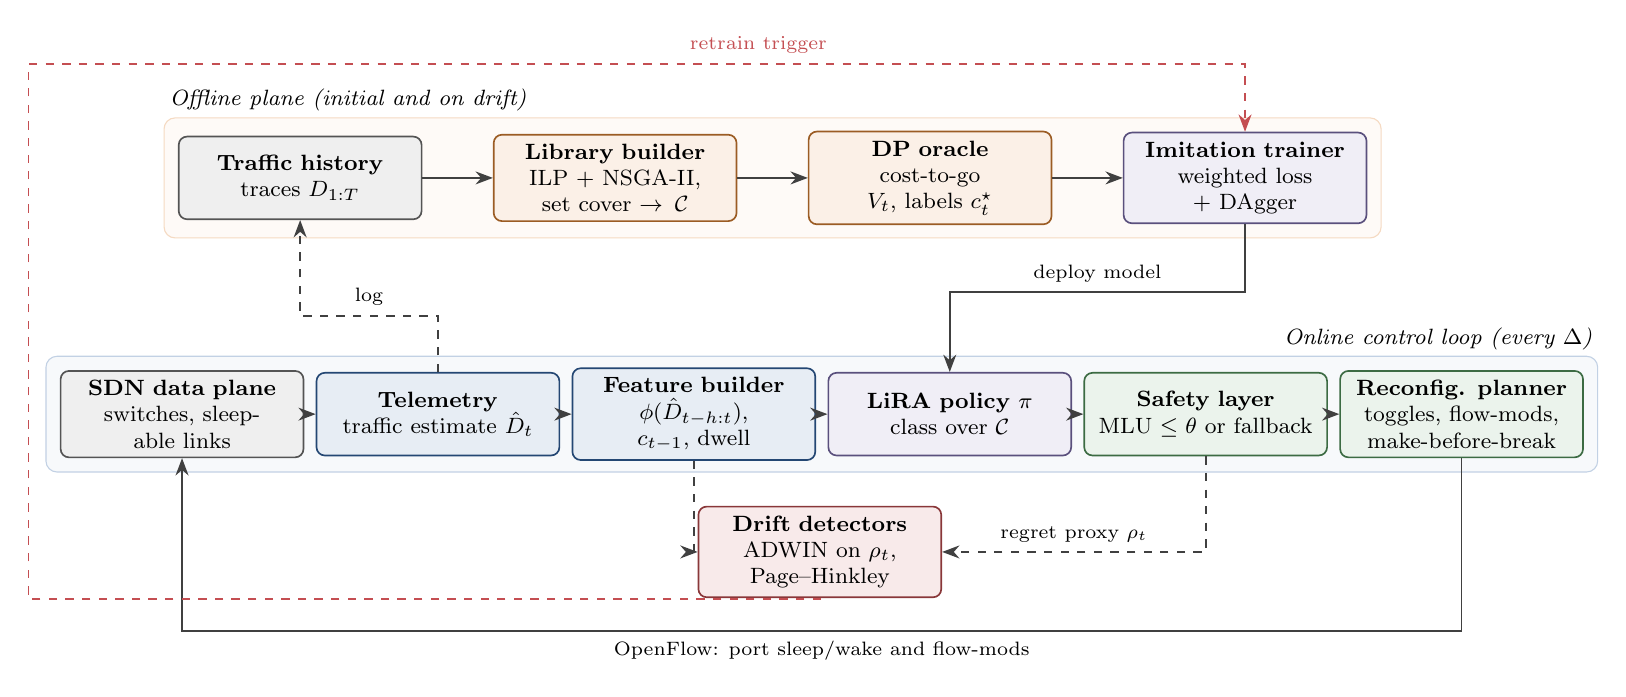
\begin{tikzpicture}
\node[box=cGray] (hist) at (1.5,3.0) {\textbf{Traffic history}\\traces $D_{1:T}$};
\node[box=cOrange] (lib) at (5.5,3.0) {\textbf{Library builder}\\ILP + NSGA-II, set cover $\rightarrow\mathcal{C}$};
\node[box=cOrange] (dp) at (9.5,3.0) {\textbf{DP oracle}\\cost-to-go $V_t$, labels $c^\star_t$};
\node[box=cPurple] (train) at (13.5,3.0) {\textbf{Imitation trainer}\\weighted loss + DAgger};
\node[box=cGray] (dpl) at (0,0) {\textbf{SDN data plane}\\switches, sleepable links};
\node[box] (tel) at (3.25,0) {\textbf{Telemetry}\\traffic estimate $\hat{D}_t$};
\node[box] (feat) at (6.5,0) {\textbf{Feature builder}\\$\phi(\hat{D}_{t-h:t})$, $c_{t-1}$, dwell};
\node[box=cPurple] (pol) at (9.75,0) {\textbf{LiRA policy} $\pi$\\class over $\mathcal{C}$};
\node[box=cGreen] (safe) at (13,0) {\textbf{Safety layer}\\$\mathrm{MLU}\le\theta$ or fallback};
\node[box=cGreen] (plan) at (16.25,0) {\textbf{Reconfig. planner}\\toggles, flow-mods, make-before-break};
\node[box=cRed] (drift) at (8.1,-1.75) {\textbf{Drift detectors}\\ADWIN on $\rho_t$, Page--Hinkley};
\begin{scope}[on background layer]
\node[fill=cOrange!4,draw=cOrange!30,rounded corners=4pt,inner sep=5pt,fit=(hist)(train),label={[font=\footnotesize\itshape,anchor=south west,inner sep=2pt]north west:Offline plane (initial and on drift)}] {};
\node[fill=cBlue!4,draw=cBlue!30,rounded corners=4pt,inner sep=5pt,fit=(dpl)(plan),label={[font=\footnotesize\itshape,anchor=south east,inner sep=2pt]north east:Online control loop (every $\Delta$)}] {};
\end{scope}
\draw[arr] (hist) -- (lib);
\draw[arr] (lib) -- (dp);
\draw[arr] (dp) -- (train);
\draw[arr] (dpl) -- (tel);
\draw[arr] (tel) -- (feat);
\draw[arr] (feat) -- (pol);
\draw[arr] (pol) -- (safe);
\draw[arr] (safe) -- (plan);
\draw[arr] (train.south) -- (13.5,1.55) -- node[above,font=\scriptsize,pos=0.5]{deploy model} (9.75,1.55) -- (pol.north);
\draw[darr] (tel.north) -- (3.25,1.25) -- node[above,font=\scriptsize]{log} (1.5,1.25) -- (hist.south);
\draw[arr] (plan.south) -- (16.25,-2.75) -- node[below,font=\scriptsize]{OpenFlow: port sleep/wake and flow-mods} (0,-2.75) -- (dpl.south);
\draw[darr] (feat.south) -- (6.5,-1.75) -- (drift.west);
\draw[darr] (safe.south) -- (13,-1.75) -- node[above,font=\scriptsize]{regret proxy $\rho_t$} (drift.east);
\draw[darr,draw=cRed] (drift.south) -- (8.1,-2.35) -- (-1.95,-2.35) -- (-1.95,4.45) -- node[above,font=\scriptsize,text=cRed,pos=0.6]{retrain trigger} (13.5,4.45) -- (train.north);
\end{tikzpicture}}
\caption{Architecture of LiRA. The offline plane builds the configuration library, computes sequence-optimal labels with the dynamic-programming oracle, and trains the policy. The online loop estimates the traffic matrix, selects a configuration conditioned on the installed one, enforces the utilization bound, and installs only the configuration difference. Drift detectors trigger retraining.}
\label{fig:arch}
\end{figure*}

\subsection{Configuration Library}\label{sec:library}

The library must be small enough for fast decisions and rich enough to contain an efficient feasible configuration for almost every traffic matrix. We cluster training traffic matrices with $k$-means ($64$ clusters) and take the element-wise 95th-percentile matrix of each cluster as its representative. For each representative we solve the path-based energy-minimization integer program with $k=4$ shortest paths, link-pair sleeping, connectivity, and the bound \eqref{eq:mlu}, and we run NSGA-II~\cite{deb2002nsga2} on port count and maximum utilization to add Pareto-diverse link-state vectors. For Abilene, whose link-state space is small, we also enumerate all connected link states. Duplicate vectors are merged, the routing of each vector is re-optimized by a linear program that minimizes maximum utilization, and further integer programs are solved for uncovered training and validation matrices until at least 99.5\% are covered. The all-on configuration is always included. The library is pruned to $K$ configurations by greedy energy coverage on every sixth training interval. Section~\ref{sec:res-bound} bounds what this restriction costs.

\subsection{Exact Sequence-Optimal Oracle}

Because all terms of \eqref{eq:objective} depend only on $(c_{t-1},c_t,D_t)$, the problem is a shortest path through a trellis whose stages are intervals and whose states are library members (Fig.~\ref{fig:trellis}). Infeasible states receive infinite cost. The backward recursion
\begin{equation}\label{eq:dp}
\begin{aligned}V_{t-1}(c')&=\min_{c\in\mathcal{C}}Q_t(c',c),\\
Q_t(c',c)&=E(c,D_t)+\lambda_R R(c',c)+\lambda_W W(c',c)+V_t(c)\end{aligned}
\end{equation}
computes the cost-to-go $V_t(c)$ of being in $c$ at the end of interval $t$, with $V_T\equiv0$. The oracle trajectory follows $c^\star_t=\arg\min_c Q_t(c^\star_{t-1},c)$. The table $Q_t(c',\cdot)$ also gives the optimal action for \emph{any} installed configuration $c'$, which we use to relabel states visited by the learner.

\begin{proposition}\label{prop:dp}
For a fixed library $\mathcal{C}$ and known $D_{1:T}$, recursion \eqref{eq:dp} returns a feasible sequence minimizing \eqref{eq:objective} whenever one exists, in $O(TK^2)$ time and $O(TK)$ memory.
\end{proposition}
\begin{proof}
By \eqref{eq:wear}, the wear contribution is a sum of terms that each depend on one pair of consecutive configurations, and \eqref{eq:energy} and \eqref{eq:reconf} depend on $(c_{t-1},c_t,D_t)$ only. Hence \eqref{eq:objective} is the length of a path through a layered graph with $K$ nodes per layer, and edges into infeasible nodes have infinite weight. Bellman's principle of optimality yields \eqref{eq:dp}, and each layer requires $K^2$ evaluations of precomputed quantities.
\end{proof}

\begin{figure}[t]
\centering
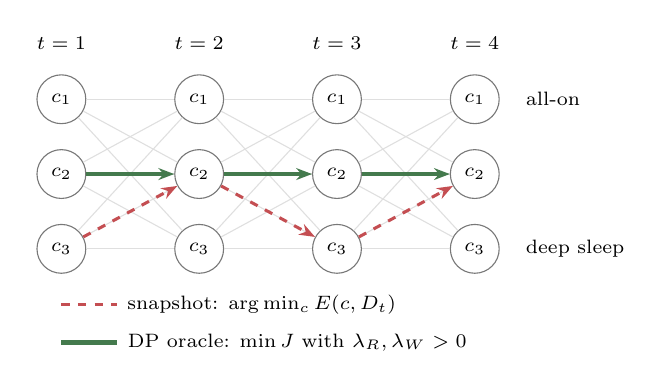
\begin{tikzpicture}[st/.style={circle,draw=cGray,fill=white,minimum size=0.62cm,inner sep=0pt,font=\scriptsize},x=1.75cm,y=0.95cm]
\foreach \t in {1,...,4}{\node[font=\scriptsize] at (\t,0.75) {$t=\t$};}
\foreach \t in {1,...,4}{\foreach \c/\y in {1/0,2/-1,3/-2}{\node[st] (n\t\c) at (\t,\y) {$c_{\c}$};}}
\foreach \t/\u in {1/2,2/3,3/4}{\foreach \a in {1,2,3}{\foreach \b in {1,2,3}{\draw[gray!25,line width=0.4pt] (n\t\a) -- (n\u\b);}}}
\draw[cRed,line width=1.1pt,dashed,-{Stealth[length=2mm]}] (n13) -- (n22);
\draw[cRed,line width=1.1pt,dashed,-{Stealth[length=2mm]}] (n22) -- (n33);
\draw[cRed,line width=1.1pt,dashed,-{Stealth[length=2mm]}] (n33) -- (n42);
\draw[cGreen!80!black,line width=1.6pt,-{Stealth[length=2mm]}] (n12) -- (n22);
\draw[cGreen!80!black,line width=1.6pt,-{Stealth[length=2mm]}] (n22) -- (n32);
\draw[cGreen!80!black,line width=1.6pt,-{Stealth[length=2mm]}] (n32) -- (n42);
\node[font=\scriptsize,anchor=west] at (4.3,0) {all-on};
\node[font=\scriptsize,anchor=west] at (4.3,-2) {deep sleep};
\draw[cRed,line width=1.1pt,dashed] (1.0,-2.75) -- (1.4,-2.75) node[right,font=\scriptsize,text=black] {snapshot: $\arg\min_c E(c,D_t)$};
\draw[cGreen!80!black,line width=1.6pt] (1.0,-3.25) -- (1.4,-3.25) node[right,font=\scriptsize,text=black] {DP oracle: $\min J$ with $\lambda_R,\lambda_W>0$};
\end{tikzpicture}
\caption{Configuration trellis (schematic). Nodes are library configurations per interval, and edges carry reconfiguration and wear costs. Snapshot selection flaps between $c_2$ and $c_3$ when traffic hovers near a decision boundary, whereas the oracle keeps $c_2$ when the extra energy is smaller than the switching cost.}
\label{fig:trellis}
\end{figure}

\subsection{History-Conditioned Policy}

The policy maps the input $s_t$ to a library index. The input contains the principal components (95\% variance, fitted on training data) of the log-scaled origin--destination vector, the total volume, the shares of the ten largest demands, time of day and day of week, the changes of the principal components and the volume over the last $1$, $3$, and $6$ intervals, the one-hot encoding of the installed configuration $c_{t-1}$, and its dwell time $\ell_{t-1}$ in intervals, capped at one day. The default model is a gradient-boosted tree classifier (XGBoost~\cite{chen2016xgboost}), and Section~\ref{sec:res-models} compares LightGBM~\cite{ke2017lightgbm}, random forests~\cite{breiman2001rf}, and a multilayer perceptron.

\textbf{Cost-sensitive imitation.} Plain classification treats all mistakes as equal, although choosing an action that is almost as cheap as the optimum is harmless. For each training state $(t,c')$ we compute the oracle action $a^\star=\arg\min_c Q_t(c',c)$ and the cost gap $g_t(c')=\min_{c\neq a^\star}Q_t(c',c)-Q_t(c',a^\star)$ to the second-best action. The classifier is trained with the sample weight $w=\mathrm{clip}(g/\bar g,0.2,5)$, where $\bar g$ is the mean gap, so that decisions with a large cost difference matter more. This weighted cross-entropy loss is a practical surrogate for a cost-sensitive classifier.

\textbf{DAgger.} A policy trained only on oracle trajectories never sees the states that its own mistakes create. We apply DAgger~\cite{ross2011dagger} with three rounds: the current policy is rolled out on the training period, with the expert action used with probability $\beta_n=0.5\cdot0.5^{\,n-1}$ in round $n$, the visited pairs $(t,c_{t-1})$ are relabeled from the stored $Q$ tables without solving any new problem, and the policy is retrained on the aggregated data. Among the rounds, we keep the policy with the lowest sequence cost on the validation period. In \daggerRoundZero\ of our \daggerRuns\ main runs this is the policy of round zero, trained on oracle trajectories alone.

\textbf{Remark.} Because the oracle's table $Q_t$ gives the optimal action from every installed configuration, the DAgger analysis for task costs~\cite{ross2011dagger} applies with a per-deviation loss of at most $u=\max_{t,c',c}[Q_t(c',c)-\min_{\tilde c}Q_t(c',\tilde c)]$, so the cost gap grows linearly in the learner's disagreement with the oracle rather than quadratically in $T$. Our weighted cross-entropy only approximates the cost-sensitive loss of that analysis, so this motivates the design and is not a guarantee for the implemented learner.

\subsection{Safety Layer}

At run time, the configuration chosen by the policy is checked against \eqref{eq:mlu} using the traffic estimate. If it is infeasible, the controller falls back to
\begin{equation}\label{eq:fallback}
\begin{split}c_t=\mathop{\arg\min}_{c\in\mathcal{C}:\,\mathrm{MLU}(c,\hat D_t)\le\theta}\Big[&E(c,\hat D_t)+\lambda_R R(c_{t-1},c)\\
&+\lambda_W W(c_{t-1},c)\Big],\end{split}
\end{equation}
which is evaluated for all $K$ configurations. If no configuration is feasible, the all-on configuration is used and the interval is counted as a violation.
\begin{proposition}\label{prop:safety}
If the all-on configuration satisfies $\mathrm{MLU}\le\theta$ for $\hat D_t$, the safety layer returns a configuration that satisfies \eqref{eq:mlu} for $\hat D_t$.
\end{proposition}
\begin{proof}
The all-on configuration belongs to $\mathcal{C}$ by construction, so the feasible set in \eqref{eq:fallback} is non-empty whenever the policy's choice is infeasible.
\end{proof}
The guarantee holds for the estimate $\hat D_t$, not for the traffic that then arrives. Section~\ref{sec:protocol} states which estimate our evaluation uses, and Section~\ref{sec:res-stale} measures the violations when the estimate is one interval old.

\subsection{Drift Detection and Retraining}\label{sec:drift}

The oracle cannot be computed online, but a myopic regret proxy can. After each decision, the controller computes
\begin{equation}\label{eq:proxy}
\begin{split}\rho_t=&E(c_t,D_t)-\min_{c\in\mathcal{C}:\,\mathrm{MLU}(c,D_t)\le\theta}E(c,D_t)\\
&+\mathbb{1}[\mathrm{MLU}(c_t,D_t)>\theta],\end{split}
\end{equation}
the energy lost against the best feasible configuration plus a violation indicator. ADWIN~\cite{bifet2007adwin} monitors $\rho_t$, and a Page--Hinkley test~\cite{page1954cusum} monitors the deseasonalized log of the total traffic volume, that is, the log volume minus its training mean for the same time of week. When a detector fires, the policy is retrained on the last seven days with oracle labels computed on that window. Because the window just after a change still contains mostly old data, retraining is repeated one and three days later. A library refresh, which adds integer-program solutions for eight clusters of the recent window, is available as an option.

\section{Algorithms}\label{sec:algorithms}

Algorithm~\ref{alg:offline} summarizes offline training and Algorithm~\ref{alg:online} the online loop. In the emulation (Section~\ref{sec:res-emu}), reconfigurations follow a make-before-break order: links that the new configuration needs are woken first, new rules are installed, and only then are unused links put to sleep. The flow-level simulation charges each change through $R$ and $W$ and does not model the transient.

\begin{algorithm}[t]
\caption{LiRA Offline Training}
\label{alg:offline}
\footnotesize
\begin{algorithmic}[1]
\Require training traces $D_{1:T}$, validation traces, prices $\lambda_R,\lambda_W$, rounds $N$
\Ensure library $\mathcal{C}$, policy $\pi$
\State $\mathcal{C}\gets$ \Call{BuildLibrary}{$D_{1:T}$} \Comment{ILP, NSGA-II, set cover}
\State precompute $E(c,D_t)$, feasibility, and $R$, $W$ for all pairs
\State compute $Q_t(c',c)$ and $V_t(c)$ by recursion \eqref{eq:dp}
\State $\mathcal{D}\gets\{(s_t,c^\star_t)\}$ on the oracle path ($s_t$ contains $c^\star_{t-1}$), weights $w$
\State train $\pi$ on $\mathcal{D}$
\For{$n=1$ to $N$}
\State roll out $\pi$ with the safety layer and expert mixing $\beta_n$; record $(t,c_{t-1})$
\State relabel the visited pairs from $Q_t(c_{t-1},\cdot)$ and add them to $\mathcal{D}$
\State retrain $\pi$ on $\mathcal{D}$
\EndFor
\State \Return $\mathcal{C}$ and the policy with the lowest validation cost
\end{algorithmic}
\end{algorithm}

\begin{algorithm}[t]
\caption{LiRA Online Control Loop}
\label{alg:online}
\footnotesize
\begin{algorithmic}[1]
\Require $\mathcal{C}$, $\pi$, threshold $\theta$, initial $c_0$
\For{each interval $t=1,2,\dots$}
\State build $s_t$ from the traffic estimate, $c_{t-1}$, and its dwell time
\State $c\gets\pi(s_t)$
\If{$\mathrm{MLU}(c,\hat D_t)>\theta$}
\State $c\gets$ fallback rule \eqref{eq:fallback}
\EndIf
\If{$c\neq c_{t-1}$}
\State wake links in $x\setminus x_{t-1}$; install new rules
\State sleep links in $x_{t-1}\setminus x$
\EndIf
\State $c_t\gets c$; observe $D_t$; update detectors with $\rho_t$ from \eqref{eq:proxy}
\If{a detector fires}
\State schedule retraining on the last seven days (Section~\ref{sec:drift})
\EndIf
\EndFor
\end{algorithmic}
\end{algorithm}

\section{Experimental Setup}\label{sec:setup}

\subsection{Datasets and Scenarios}

Table~\ref{tab:data} lists the data. Abilene (Zhang \emph{et al.}~\cite{zhang2003tomogravity}) and G\'{E}ANT (Uhlig \emph{et al.}~\cite{uhlig2006geant}) topologies and traffic matrices come from SNDlib~\cite{orlowski2010sndlib}. SNDlib offers only one day of five-minute matrices for Nobel-Germany, while day-of-week features and a chronological split need several weeks. We therefore generate a 30-day semi-synthetic series: a gravity model fitted to the SNDlib day is modulated by the weekly profile of Abilene and multiplied by independent log-normal noise per origin--destination pair and interval, whose scale ($\sigma=1.23$) is fitted to the residuals of Abilene. This noise has no temporal correlation and is therefore harsher than the noise of a real trace.

We removed unfilled gaps and all-zero measurement outages, interpolated gaps of up to three intervals, removed eleven G\'{E}ANT intervals whose total volume exceeds ten times its one-day rolling median, and split each series chronologically into 60\% training, 15\% validation, and 25\% test. Sequences never cross an unfilled gap. Traffic is scaled so that the 99.9th percentile of the all-on maximum link utilization on the training split is $0.5$, which makes the scenario ``base''.

We add three scenarios to probe regimes in which sequence decisions could matter more: \emph{high load} (demands $\times1.6$, a training peak of $0.8$), \emph{high dynamic power} (the load-proportional port power tripled to $15$\,W), and \emph{stress} (both). The library is rebuilt for each scenario.

\begin{table*}[t]
\centering
\caption{Topologies and Traffic Data}
\label{tab:data}
\footnotesize
\setlength{\tabcolsep}{2.5pt}
\begin{adjustbox}{max width=\textwidth}\begin{tabular}{@{}lcccccc@{}}
\toprule
Topology & $|V|$ & $|E|$ & $\Delta$ & Intervals & Span & Traffic \\
\midrule
Abilene & 12 & 15 & 5\,min & 48\,108 & 2004-03-01 to 2004-09-10 & real (SNDlib) \\
G\'{E}ANT & 22 & 36 & 15\,min & 10\,784 & 2005-05-04 to 2005-08-31 & real (SNDlib) \\
Nobel-Germany & 17 & 26 & 5\,min & 8\,640 & 2004-03-01 to 2004-03-30 & semi-synthetic \\
\bottomrule
\end{tabular}
\end{adjustbox}
\end{table*}

\subsection{Baselines}

B0 keeps all links on and routes each demand on its shortest path. B4 is our reimplementation of the snapshot-learning principle~\cite{gomezdelahiz2025noms,gomezdelahiz2026tgcn}: an XGBoost classifier that maps the current traffic features to the energy-optimal feasible library member. If its choice violates $\theta$, B4 falls back to the feasible configuration with the lowest energy. B6 applies hysteresis to B4, switching only if the energy gain of the proposed configuration exceeds a threshold, and B7 applies a minimum dwell time. Both thresholds are tuned on the validation split by sequence cost $J$. B2 is a rolling-horizon controller that solves the sequential problem exactly over the library for the next 12 intervals with a persistence forecast and applies the first action. It needs no learning and is restricted to the library. The static rule holds the configuration that the oracle uses most often on the training period and applies LiRA's fallback \eqref{eq:fallback} whenever that configuration is infeasible. It is LiRA with its classifier replaced by a constant. B1 solves the energy integer program for each traffic matrix with HiGHS~\cite{huangfu2018highs}, B3 runs NSGA-II per traffic matrix, and B5 is an ElasticTree-style greedy heuristic~\cite{heller2010elastictree}. B1, B3, and B5 are evaluated on a subsample of 60 test intervals (15 for B3 on Abilene) because of their run time. We also report the offline oracle $\mathrm{O}^\star$, which uses the future and is a lower bound for every controller restricted to the library. Section~\ref{sec:res-bound} bounds controllers that are not. A deep reinforcement learning baseline is not included.

\subsection{Information Available to the Controller}\label{sec:protocol}

Unless stated otherwise, every online method chooses the configuration of interval $t$ with the realized matrix $D_t$: its features are computed from $D_t$, and its safety check uses $\mathrm{MLU}(c,D_t)$. This idealizes the estimate $\hat D_t$ of Algorithm~\ref{alg:online}, and it gives the safety layer the information that the oracle has. Section~\ref{sec:res-stale} repeats the comparison when every online method decides with $D_{t-1}$, the last completed measurement, with and without a safety margin of $0.05$ on $\theta$.

\subsection{Metrics and Prices}

Energy savings $S$ are measured relative to B0. We report configuration changes and link power-state transitions per day, flow-modification messages, the share of intervals with a violation of $\theta$, the sequence cost $J$ of \eqref{eq:objective}, the mean and maximum acceleration factor, and the decision latency measured with batch size one. The retention $X=S_{\mathrm{LiRA}}/S_{\mathrm{B4}}$ and the reductions $Y=1-N^{\mathrm{ch}}_{\mathrm{LiRA}}/N^{\mathrm{ch}}_{\mathrm{B4}}$ and $Z=1-N^{\mathrm{tr}}_{\mathrm{LiRA}}/N^{\mathrm{tr}}_{\mathrm{B4}}$ are defined only when B4 changes configuration. The reported cost $J$ is \eqref{eq:objective} without the constraint: an interval that violates $\theta$ adds no penalty and is counted in the violation share instead, and the first test interval and the first interval after a measurement gap carry no switching cost. $J$ also includes the modeled wear credit of sleeping links, so it is not an energy figure: absolute values of $J$ are lower than the energy of the always-on network, and only differences between methods are meaningful. With the default prices a sleeping link earns a wear credit of \wearCredit\ per interval, while sleeping it saves \sleepSaveabi, \sleepSavenob, and \sleepSavegea\ of the normalized energy on Abilene, Nobel-Germany, and G\'{E}ANT, so the wear model rewards sleeping about as much as the energy model does.

The prices are set from operating considerations. One typical large change costs $0.2\%$ of the daily energy of the all-on network, so $\lambda_R=0.002\,n_d$, and one link transition costs $0.08\%$ of it, so $\lambda_W=0.0008\,n_d/\chi$, where $n_d$ is the number of intervals per day. For stochastic components (classifier seeds and DAgger rollouts) we use five seeds and report means with 95\% confidence intervals. Where a policy is constant, all seeds give the same result and the confidence interval has zero width. We compare the per-day sequence costs of LiRA with those of B4, B6, and B7 with the Wilcoxon signed-rank test and correct the three comparisons per setting with the Holm method. Because twelve settings are tested, we also apply the Holm correction to all \globalTests\ comparisons at once and report the result. Confidence intervals that round to zero, which occur when every seed gives the same sequence, are not printed.

\subsection{Implementation and Parameters}\label{sec:params}

The flow-level simulator is written in Python with NumPy and sparse path--link matrices. Integer and linear programs are solved with HiGHS (highspy 1.15.1). Experiments ran on an Intel Core i9-13900H laptop (14 cores, 20 threads, 48\,GB RAM, no GPU) under Windows, and the emulation ran in Ubuntu on WSL2 with Mininet 2.3.0 and Open vSwitch 3.7.1. Table~\ref{tab:params} lists the parameters. The port power values are representative assumptions within the ranges reported in~\cite{vishwanath2014modeling,mahadevan2009power}, not measurements of a specific device, and the wear parameters are assumed values for the model of~\cite{chiaraviglio2015lifetime}. We therefore study the sensitivity to both (Section~\ref{sec:res-wear}).

\begin{table}[t]
\centering
\caption{Model and Training Parameters}
\label{tab:params}
\footnotesize
\setlength{\tabcolsep}{3pt}
\begin{tabular}{@{}p{3.9cm}p{4.6cm}@{}}
\toprule
Parameter & Value \\
\midrule
Threshold $\theta$; paths $k$; library $K$ & 0.8; 4; 32 (default) \\
Port power $P^{\mathrm{idle}}$/$P^{\mathrm{dyn}}$/$P^{\mathrm{sl}}$ & 30/5/3\,W \\
Wear $\alpha$; $\chi$ & 0.5; 0.01 per transition per day \\
Prices $\lambda_R$; $\lambda_W$ & $0.002\,n_d$; $0.0008\,n_d/\chi$ \\
Interval $\Delta$; $n_d$ & 5\,min, 288 (G\'{E}ANT: 15\,min, 96) \\
XGBoost & depth 6, rate 0.1, 150 rounds max, early stop 15 \\
Features & PCA 95\% variance, lags 1/3/6 \\
DAgger rounds; $\beta_1$; weight clip & 3; 0.5; $[0.2,5]$ \\
ADWIN confidence; Page--Hinkley tolerance, forgetting & 0.002; 0.005, 0.9999 \\
Retraining window; schedule & 7 days; at detection, $+1$ and $+3$ days \\
Seeds; folds & 5; 4 rolling origins \\
\bottomrule
\end{tabular}
\end{table}

\section{Results}\label{sec:results}

Two facts about the trained LiRA policies frame all results. In \liraConstRuns\ of the \liraTotalRuns\ main runs (all Abilene runs and the Nobel-Germany base and high-dynamic-power scenarios) the trained policy is a constant classifier, because the oracle uses a single configuration on the training period. LiRA then holds the configuration that was optimal on the training period and switches only through its fallback, and its ablations are trivial. In \daggerRoundZero\ of the \daggerRuns\ runs the policy selected on validation data is that of round zero, before any DAgger data. The static rule of Section~\ref{sec:setup} makes the consequence measurable: it reaches the same cost as LiRA in \staticSame\ of the \staticTotal\ settings of Table~\ref{tab:scen}.

\subsection{Do Real Traces Need Sequence Awareness?}\label{sec:res-main}

Table~\ref{tab:main} gives the main comparison in the base scenario. On Abilene and G\'{E}ANT, B4, B6, B7, LiRA, and the oracle reach the same energy savings (\abiSav\% and \geaSav\%), make at most \abiBFourchg\ configuration changes per day, and have sequence costs within \realSpread\% of each other. The rolling-horizon controller B2, which relies on a persistence forecast, is marginally worse on Abilene. The oracle itself uses a single configuration for the whole test period (\abiTestDays\ and \geaTestDays\ days). B4 never changes configuration on G\'{E}ANT, so the reductions $Y$ and $Z$ are undefined there, and on Abilene they would rest on less than one change on average over the test period. LiRA is no worse and no better. The per-day cost differences between LiRA and B4, B6, and B7 are not significant on these traces (Table~\ref{tab:scen}).

\begin{table*}[t]
\centering
\caption{Main Comparison in the Base Scenario (Test Split). Means with 95\% Confidence Intervals over Five Seeds for B4, B6, B7, and LiRA; Single Values Otherwise. Latency Is the Median Decision Time}
\label{tab:main}
\footnotesize
\setlength{\tabcolsep}{4pt}
\begin{adjustbox}{max width=\textwidth}\begin{tabular}{@{}lccccccc@{}}
\toprule
Method & $S$ (\%) & Changes/d & Transitions/d & MLU viol. (\%) & $J$ & $\overline{\mathrm{AF}}$ & Latency (ms) \\
\midrule
\multicolumn{8}{@{}l}{\textit{Abilene}} \\
B0 always-on & 0.00 & 0.00 & 0.00 & 0.00 & 12037.5 & 1.000 & -- \\
B4 snapshot ML & 23.98 & 0.02$\pm$0.05 & 0.08$\pm$0.21 & 0.00 & 7227.7$\pm$2.8 & 0.867 & 0.989 \\
B6 B4+hysteresis & 23.98 & 0.00 & 0.00 & 0.00 & 7226.7 & 0.867 & 0.989 \\
B7 B4+min-dwell & 23.98 & 0.02$\pm$0.05 & 0.08$\pm$0.21 & 0.00 & 7227.7$\pm$2.8 & 0.867 & 0.989 \\
B2 rolling horizon & 23.95 & 0.00 & 0.00 & 0.00 & 7230.4 & 0.867 & 0.433 \\
LiRA & 23.98 & 0.00 & 0.00 & 0.00 & 7226.7 & 0.867 & 0.008 \\
Oracle O$^\star$ & 23.98 & 0.00 & 0.00 & 0.00 & 7226.7 & 0.867 & -- \\
\midrule
\multicolumn{8}{@{}l}{\textit{G\'{E}ANT}} \\
B0 always-on & 0.00 & 0.00 & 0.00 & 0.00 & 2705.2 & 1.000 & -- \\
B4 snapshot ML & 29.85 & 0.00 & 0.00 & 0.00 & 603.7 & 0.833 & 1.599 \\
B6 B4+hysteresis & 29.85 & 0.00 & 0.00 & 0.00 & 603.7 & 0.833 & 1.599 \\
B7 B4+min-dwell & 29.85 & 0.00 & 0.00 & 0.00 & 603.7 & 0.833 & 1.599 \\
B2 rolling horizon & 29.85 & 0.00 & 0.00 & 0.00 & 603.7 & 0.833 & 0.432 \\
LiRA & 29.85 & 0.00 & 0.00 & 0.00 & 603.7 & 0.833 & 1.571 \\
Oracle O$^\star$ & 29.85 & 0.00 & 0.00 & 0.00 & 603.7 & 0.833 & -- \\
\midrule
\multicolumn{8}{@{}l}{\textit{Nobel-Germany}} \\
B0 always-on & 0.00 & 0.00 & 0.00 & 0.05 & 2163.7 & 1.000 & -- \\
B4 snapshot ML & 27.63 & 11.68$\pm$0.89 & 23.36$\pm$1.78 & 0.00 & 931.7$\pm$4.3 & 0.855$\pm$0.001 & 0.949 \\
B6 B4+hysteresis & 27.63 & 0.13 & 0.27 & 0.00 & 875.3 & 0.846 & 0.949 \\
B7 B4+min-dwell & 27.63 & 2.29$\pm$0.18 & 4.59$\pm$0.36 & 0.00 & 885.8$\pm$0.9 & 0.848 & 0.949 \\
B2 rolling horizon & 27.63 & 0.13 & 0.27 & 0.00 & 875.3 & 0.846 & 0.423 \\
LiRA & 27.63 & 0.27 & 0.53 & 0.00 & 875.9 & 0.846 & 0.008 \\
Oracle O$^\star$ & 27.63 & 0.00 & 0.00 & 0.00 & 874.7 & 0.846 & -- \\

\bottomrule
\end{tabular}
\end{adjustbox}
\end{table*}

The Nobel-Germany series behaves differently. B4 changes configuration \nobBFourchg\ times per day and makes \nobBFourtrans\ link transitions per day, whereas the exact snapshot rule \eqref{eq:snapshot} would change \nobSnapChg\ times per day. LiRA makes \nobLiRAchg\ changes per day, a reduction of $Y=\nobY\%$ and $Z=\nobZ\%$ at an energy retention of $X=\nobX\%$, and the mean acceleration factor drops from \nobAFfour\ for B4 to \nobAFlira. The reduction does not come from learning. The policy is constant in this scenario and holds one configuration in \liraHold\ of the \nobTestIntervals\ test intervals, and the static rule gives the same result. Hysteresis (B6) and the rolling-horizon B2 both make \nobBsixChg\ changes per day at a cost of \nobJBsixbase, slightly below LiRA's \nobJLiRAbase, so LiRA is not better than either. The paired test gives an adjusted $p=\nobPbsix$ against B6, with a mean daily cost difference (LiRA minus B6) of \effBsixbase\ and LiRA cheaper on \effBsixDaysbase\% of the days, and $p=\nobPbfour$ against B4. These reductions are relative to a gradient-boosted B4 that flaps heavily. A random-forest B4 changes configuration only \modRfChg\ times per day (Section~\ref{sec:res-models}), so the size of $Y$ and $Z$ depends on the classifier that we reimplemented. The test uses eight daily samples, the last of them a half day, so the smallest attainable two-sided $p$-value is $0.0078$. With the Holm correction over all \globalTests\ comparisons of Table~\ref{tab:scen}, \globalSig\ remain significant (smallest adjusted $p=\globalMinP$), including the comparison with B4. The cost differences we report are therefore descriptive. Their consistency across seeds, folds (Section~\ref{sec:res-folds}), and noise variants (Section~\ref{sec:res-noise}) carries more weight than any single test.

Fig.~\ref{fig:gain} shows that the flapping is harmless to remove. Among the \gainChanges\ configuration changes of B4 (seed 0) in the test period, none saves more than \gainMax\% of the interval energy, \gainTenthShare\% save less than 0.1\%, and the median saving is below \gainMedianBelow\%. Such changes are expected when demand hovers near the boundary between two nearly equivalent configurations, and avoiding them costs essentially no energy.

\begin{figure}[t]
\centering
\begin{tikzpicture}
\begin{axis}[width=\columnwidth,height=4.0cm,ybar,bar width=14pt,ymin=0,ymax=110,ylabel={Share of changes (\%)},xlabel={Energy saved by a change (\% of interval energy)},xtick=data,xticklabels={$<0.1$,0.1--0.5,0.5--1,1--2,$>2$},nodes near coords={\pgfmathprintnumber[fixed,precision=0]{\pgfplotspointmeta}},nodes near coords style={font=\scriptsize},enlarge x limits=0.15]
\addplot[fill=cRed!55,draw=cRed] table[x=bin,y=share,col sep=space]{generated/gain_hist.dat};
\end{axis}
\end{tikzpicture}
\caption{Energy gained by each configuration change of the snapshot classifier B4 (seed 0) on the Nobel-Germany test period (\gainChanges\ changes). \gainTenthShare\% of the changes save less than 0.1\% of the interval energy.}
\label{fig:gain}
\end{figure}

\subsection{Other Scenarios and Where the Differences Come From}

Table~\ref{tab:scen} summarizes all topologies and scenarios. Higher load and higher dynamic power change nothing on Abilene and G\'{E}ANT: the oracle remains a single configuration. On Nobel-Germany, higher load makes the optimal sequence non-constant (\nobhlOchg\ changes per day). B4 then makes \nobhlBFourchg\ changes per day, B6 makes \nobhlBsixChg, and LiRA makes \nobhlLiRAchg. LiRA's sequence equals the oracle's in every test interval and every seed (\hlLiraOracleDiff\ differing intervals), at a cost of \nobJLiRAhl\ against \nobJBtwohl\ for B2, \nobJBsixhl\ for B6, and \nobhlJBFour\ for B4. The match has a simple cause. The expert is nearly constant, LiRA predicts the default configuration, and its safety layer, which sees the realized matrix, switches in exactly the intervals in which the default becomes infeasible, as the oracle does. The static rule reaches the same cost (\staticJhl), and so does every ablation that keeps the safety layer (Section~\ref{sec:res-ablation}). Over \nobTestDays\ days of test data the difference to B6 is not significant ($p=\nobhlPbsix$, LiRA cheaper on \effBsixDayshl\% of the days). Under stress, the only setting in which LiRA differs from the static rule, LiRA (\nobJLiRAst) is cheaper in total than B6 (\nobJBsixst) and the static rule (\staticJst), but B2 (\nobJBtwost) comes closer to the oracle (\nobJOst). The difference to B6 is \nobstGainPct\% of the cost, LiRA is cheaper on only \nobstBsixDays\% of the days, and the test gives $p=\nobstPbsix$.

\begin{table*}[t]
\centering
\caption{All Topologies and Scenarios: Configuration Changes per Day, Total Cost $J$, and Holm-Adjusted $p$-Values of the Wilcoxon Test on Per-Day Cost (B4, B6, and LiRA: Mean over Five Seeds)}
\label{tab:scen}
\footnotesize
\setlength{\tabcolsep}{3.5pt}
\begin{adjustbox}{max width=\textwidth}\begin{tabular}{@{}llccccccccccc@{}}
\toprule
 & & \multicolumn{4}{c}{Changes/d} & \multicolumn{5}{c}{Total cost $J$} & \multicolumn{2}{c}{$p_{\mathrm{Holm}}$} \\
\cmidrule(lr){3-6}\cmidrule(lr){7-11}\cmidrule(lr){12-13}
Topology & Scenario & B4 & B6 & B2 & LiRA & B4 & B6 & B2 & LiRA & O$^\star$ & vs B4 & vs B6 \\
\midrule
Abilene & base & 0.02 & 0.00 & 0.00 & 0.00 & 7227.7 & 7226.7 & 7230.4 & 7226.7 & 7226.7 & 0.539 & 1.000 \\
Abilene & high load & 0.00 & 0.00 & 0.02 & 0.00 & 7233.0 & 7233.0 & 7237.2 & 7233.0 & 7233.0 & 1.000 & 1.000 \\
Abilene & high dynamic power & 0.02 & 0.00 & 0.00 & 0.00 & 7248.7 & 7247.7 & 7258.7 & 7247.7 & 7247.7 & 0.539 & 1.000 \\
Abilene & stress & 0.00 & 0.00 & 0.02 & 0.00 & 7266.6 & 7266.6 & 7277.7 & 7266.6 & 7266.6 & 1.000 & 1.000 \\
\midrule
G\'{E}ANT & base & 0.00 & 0.00 & 0.00 & 0.00 & 603.7 & 603.7 & 603.7 & 603.7 & 603.7 & 1.000 & 1.000 \\
G\'{E}ANT & high load & 0.00 & 0.00 & 0.00 & 0.00 & 610.4 & 610.4 & 610.4 & 610.4 & 610.4 & 1.000 & 1.000 \\
G\'{E}ANT & high dynamic power & 0.00 & 0.00 & 0.00 & 0.00 & 625.0 & 625.0 & 625.0 & 625.0 & 625.0 & 1.000 & 1.000 \\
G\'{E}ANT & stress & 0.00 & 0.00 & 0.00 & 0.00 & 644.8 & 644.8 & 644.8 & 644.8 & 644.8 & 1.000 & 1.000 \\
\midrule
Nobel-Germany & base & 11.68 & 0.13 & 0.13 & 0.27 & 931.7 & 875.3 & 875.3 & 875.9 & 874.7 & 0.023 & 0.875 \\
Nobel-Germany & high load & 1.76 & 1.07 & 0.93 & 0.80 & 890.7 & 887.0 & 882.2 & 880.9 & 880.9 & 0.117 & 0.312 \\
Nobel-Germany & high dynamic power & 11.68 & 0.27 & 0.13 & 0.27 & 939.5 & 883.7 & 883.2 & 883.7 & 882.9 & 0.023 & 1.000 \\
Nobel-Germany & stress & 1.76 & 1.07 & 0.93 & 0.91 & 903.1 & 899.4 & 895.4 & 898.6 & 894.3 & 0.164 & 0.641 \\

\bottomrule
\end{tabular}
\end{adjustbox}
\end{table*}

Fig.~\ref{fig:case} shows the busiest test week of the Nobel-Germany series. B4 changes configuration \caseBFourchg\ times during the week, whereas LiRA makes only \caseLiRAchg\ changes. Fig.~\ref{fig:pareto} plots total cost against configuration changes for the hysteresis and dwell-time sweeps and for the price sweep of LiRA and the oracle. LiRA and the oracle lie at the low-cost, low-change end of the plotted points, and a tuned hysteresis threshold reaches nearly the same point.

\begin{figure}[t]
\centering
\begin{tikzpicture}
\begin{axis}[width=\columnwidth,height=4.2cm,xlabel={Day of the busiest test week},ylabel={Configuration index},ymin=-0.3,ymax=3.4,legend pos=north east,legend columns=3,mark size=0.8pt]
\addplot[const plot,cRed,thick] table[x=day,y expr=\thisrow{B4}+0.0,col sep=space]{generated/case_week.dat};
\addlegendentry{B4}
\addplot[const plot,cGreen!70!black,thick] table[x=day,y expr=\thisrow{B6}+0.12,col sep=space]{generated/case_week.dat};
\addlegendentry{B6 (+0.12)}
\addplot[const plot,cBlue,thick,dashed] table[x=day,y expr=\thisrow{LiRA}+0.24,col sep=space]{generated/case_week.dat};
\addlegendentry{LiRA (+0.24)}
\end{axis}
\end{tikzpicture}
\caption{Installed configuration index over the busiest test week of the Nobel-Germany series. Offsets separate the lines. B4 switches repeatedly between two configurations, whereas B6 and LiRA hold a configuration.}
\label{fig:case}
\end{figure}

\begin{figure}[t]
\centering
\begin{tikzpicture}
\begin{groupplot}[group style={group size=2 by 1,horizontal sep=1.3cm},width=0.46\columnwidth,height=4.3cm,xmode=log,xlabel={Changes/day $+0.05$},scaled y ticks=false]
\nextgroupplot[title={Base},ylabel={Total cost $J$}]
\addplot[only marks,mark=square*,cGreen!70!black] table[x expr=\thisrow{config_changes_per_day}+0.05,y=total_cost_J,col sep=space]{generated/pareto_base_B6.dat};
\addplot[only marks,mark=triangle*,cOrange] table[x expr=\thisrow{config_changes_per_day}+0.05,y=total_cost_J,col sep=space]{generated/pareto_base_B7.dat};
\addplot[only marks,mark=*,cBlue,mark size=2pt] table[x expr=\thisrow{config_changes_per_day}+0.05,y=total_cost_J,col sep=space]{generated/pareto_base_LiRA.dat};
\addplot[only marks,mark=x,black,mark size=3pt] table[x expr=\thisrow{config_changes_per_day}+0.05,y=total_cost_J,col sep=space]{generated/pareto_base_Ostar.dat};
\addplot[only marks,mark=diamond*,cRed,mark size=3pt] table[x expr=\thisrow{config_changes_per_day}+0.05,y=total_cost_J,col sep=space]{generated/pareto_base_B4.dat};
\nextgroupplot[title={High load}]
\addplot[only marks,mark=square*,cGreen!70!black] table[x expr=\thisrow{config_changes_per_day}+0.05,y=total_cost_J,col sep=space]{generated/pareto_highload_B6.dat};
\addlegendentry{B6 sweep}
\addplot[only marks,mark=triangle*,cOrange] table[x expr=\thisrow{config_changes_per_day}+0.05,y=total_cost_J,col sep=space]{generated/pareto_highload_B7.dat};
\addlegendentry{B7 sweep}
\addplot[only marks,mark=*,cBlue,mark size=2pt] table[x expr=\thisrow{config_changes_per_day}+0.05,y=total_cost_J,col sep=space]{generated/pareto_highload_LiRA.dat};
\addlegendentry{LiRA}
\addplot[only marks,mark=x,black,mark size=3pt] table[x expr=\thisrow{config_changes_per_day}+0.05,y=total_cost_J,col sep=space]{generated/pareto_highload_Ostar.dat};
\addlegendentry{O$^\star$}
\addplot[only marks,mark=diamond*,cRed,mark size=3pt] table[x expr=\thisrow{config_changes_per_day}+0.05,y=total_cost_J,col sep=space]{generated/pareto_highload_B4.dat};
\addlegendentry{B4}
\end{groupplot}
\end{tikzpicture}
\caption{Total cost versus configuration changes on Nobel-Germany. Hysteresis thresholds and dwell times are swept for B6 and B7 and the reconfiguration price is swept for LiRA and the oracle. Each marker is one setting on the test split. The horizontal axis is logarithmic, and 0.05 is added to the change rate so that methods without changes can be shown.}
\label{fig:pareto}
\end{figure}

\subsection{Dependence on the Snapshot Classifier}\label{sec:res-models}

The amount of flapping depends strongly on the classifier. On Nobel-Germany in the base scenario, B4 with XGBoost changes configuration \modXgbChg\ times per day, LightGBM \modLgbmChg, a random forest \modRfChg, and a multilayer perceptron \modMlpChg\ (Table~S1 (Supplementary Material)). The random forest is nearly as stable as LiRA. Averaging over trees is a plausible reason, which we did not test. The perceptron flaps so much that its cost (\modMlpJ) is far above that of LiRA (\nobJlira). LiRA reaches the same cost with every backend, because its policy is constant in this scenario. A sequence-aware method is therefore most useful when the snapshot classifier is the kind that flaps, and it is least useful when a smoother classifier or a hysteresis guard is available.


\subsection{Ablation, Library Size, and Threshold}\label{sec:res-ablation}

Table~S2 (Supplementary Material) removes one component of LiRA at a time on Nobel-Germany at the default price. It uses seeds 0 to 2, so the full policy's stress cost differs from the five-seed value in Table~\ref{tab:scen}. In the high-load scenario the expert is nearly constant, so all variants that keep the safety layer reach the oracle cost. In the stress scenario the full policy costs \ablStressFull\ against \ablStressO\ for the oracle. Removing the previous-configuration input raises the cost to \ablStressNoPrev, removing the cost-sensitive weights to \ablStressNoCS, and removing DAgger to \ablStressNoDagger. Removing the lag features lowers it to \ablStressNoLag. The differences are small and of mixed sign, and we did not test them for significance. Removing the safety layer lowers the cost to \ablStressNoSafe\ because the policy then ignores the bound, and it causes \ablStressNoSafeViol\% of the intervals to violate $\theta$. Because $J$ carries no penalty for violations, this cost is not comparable, and the layer is needed. On Abilene and G\'{E}ANT all variants coincide with the oracle because the expert is constant.


Table~S3 (Supplementary Material) shows the effect of the library size on Nobel-Germany. Requested sizes above \KactualMax\ yield the same library, because the candidate pool contains only \nobCand\ configurations. Every library size covers all test matrices. A larger library lowers the cost of B4 (from \KBFouratEight\ at $K=8$ to \KBFouratSixFour\ at the largest size), but hysteresis and LiRA stay within 0.2\% of the oracle cost at every size. Table~S4 (Supplementary Material) varies the utilization threshold. At $\theta=0.6$ B4 changes configuration \thSixBFourchg\ times per day and LiRA \thSixLiRAchg\ times. For $\theta\ge0.7$, each method gives the same result at every threshold on Nobel-Germany, because the same configurations are optimal and feasible. Table~S4 (Supplementary Material) uses seed 0, so its B4 change rate differs from the five-seed mean of Table~\ref{tab:main}. On Abilene and G\'{E}ANT, the threshold has no effect between 0.6 and 0.9. LiRA never violates the bound when the library covers the traffic.



\subsection{Wear and Lifetime}\label{sec:res-wear}

Fig.~\ref{fig:wear} shows the mean acceleration factor of the decision sequences on Nobel-Germany for $\alpha=0.5$ and varying cycling weight $\chi$ (the sequences are fixed, and only the model changes). Every method stays below the always-on value of one for $\alpha=0.5$ and all $\chi$ up to $0.1$, but B4 degrades fastest: at $\chi=0.1$ its mean factor is \wearBigChiBFour, against \wearBigChiLiRA\ for LiRA. At the default parameters (seed 0) the most-cycled link of B4 has a factor of \maxAFfour, whereas the most-cycled link of LiRA has \maxAFlira\ and those of B6, B7, and the oracle \maxAFothers. When sleeping brings no benefit ($\alpha=1$), every transition lowers lifetime, and every method that switches exceeds the always-on factor, B4 by the largest margin. Absolute lifetime figures depend on assumed parameters and should be read as relative comparisons.

\begin{figure}[t]
\centering
\begin{tikzpicture}
\begin{axis}[width=\columnwidth,height=4.2cm,xmode=log,xlabel={Cycling weight $\chi$ (per transition per day)},ylabel={Mean $\mathrm{AF}$},legend pos=north west,legend columns=2,ymin=0.8,ymax=1.05]
\addplot[cRed,thick,mark=*,mark size=1.5pt] table[x=chi,y=B4,col sep=space]{generated/wear_chi.dat};\addlegendentry{B4}
\addplot[cGreen!70!black,thick,mark=square*,mark size=1.5pt] table[x=chi,y=B6,col sep=space]{generated/wear_chi.dat};\addlegendentry{B6}
\addplot[cBlue,thick,dashed,mark=triangle*,mark size=1.5pt] table[x=chi,y=LiRA,col sep=space]{generated/wear_chi.dat};\addlegendentry{LiRA}
\addplot[black,dotted,thick] table[x=chi,y=B0,col sep=space]{generated/wear_chi.dat};\addlegendentry{Always on}
\end{axis}
\end{tikzpicture}
\caption{Mean acceleration factor of the decision sequences on Nobel-Germany for $\alpha=0.5$. The factor of the always-on network is one.}
\label{fig:wear}
\end{figure}

\subsection{Decision Time and Scalability}\label{sec:res-time}

The library-based decisions are fast. The median decision time of B4 is \abiLatBFour\,ms on Abilene, \nobLatBFour\,ms on Nobel-Germany, and \geaLatBFour\,ms on G\'{E}ANT. LiRA needs less than 0.01\,ms where its policy is constant and \geaLatLiRA\,ms where a tree model is evaluated. The safety check takes at most \safetyTA\,ms even on a 65-node topology. Solving the integer program per traffic matrix (B1) takes a median of \nobIlpMs\,ms on Nobel-Germany and \geaIlpS\,s on G\'{E}ANT, NSGA-II (B3) takes \nobGaS\,s and \geaGaS\,s, and the greedy heuristic is faster but gives away part of the savings (Table~S5 (Supplementary Material)). On the subsample, the per-snapshot integer program reaches the same savings as the library snapshot optimum to within \boneGapPP\ percentage points. On larger SNDlib topologies the integer program takes \ilpGermany\,s for Germany50 and \ilpTA\,s for TA2 (Table~S6 (Supplementary Material)). These times fit five-minute intervals on the topologies we study, so speed alone does not require a learned controller here. The dynamic-programming oracle needs \dpRunAbi\,s for all \abiIntervals\ Abilene intervals with $K=32$, so prices can be explored offline.



\subsection{What the Library Gives Up}\label{sec:res-bound}

Because the switching terms of \eqref{eq:objective} are non-negative, the sum over the test intervals of the optimal single-interval cost, with free link states and free routing over the $k$ paths, is a lower bound on the cost $J$ of any controller, with or without a library, including the optimum of the full multi-period mixed-integer program. We solve this single-interval integer program with HiGHS for \boundAllOptimal\ \boundIntervals\ test intervals of five settings (median \boundMedianMs\,ms per interval, largest relative gap $\boundMaxMipGap$) and use the solver's dual bound. Table~\ref{tab:bound} compares the bound with the library snapshot optimum, which picks the best library member in every interval and also ignores switching, with the oracle, and with LiRA. The library restriction itself costs at most \boundMaxLoss\% in any setting. The oracle lies within \boundMaxGap\% of the bound, and on Nobel-Germany under high load and stress most of that gap is the cost of holding a configuration instead of re-optimizing every interval, which the bound ignores. A multi-period program without a library can therefore improve on the oracle by at most \boundMaxGap\%.

\begin{table}[t]
\centering
\caption{Lower Bound on the Cost of Any Controller (Sum of Per-Interval Optima), the Library Snapshot Optimum, the Oracle, and LiRA on the Test Split. Library Loss Is the Snapshot Optimum Above the Bound, O$^\star$ Gap the Oracle Above the Bound, Both Relative to the Oracle Cost}
\label{tab:bound}
\scriptsize
\setlength{\tabcolsep}{2pt}
\begin{adjustbox}{max width=\textwidth}\begin{tabular}{@{}lcccccc@{}}
\toprule
Setting & Bound & Lib. snapshot & O$^\star$ & LiRA & Lib. loss (\%) & O$^\star$ gap (\%) \\
\midrule
Abilene & 7226.7 & 7226.7 & 7226.7 & 7226.7 & 0.000 & 0.000 \\
G\'{E}ANT & 603.7 & 603.7 & 603.7 & 603.7 & 0.011 & 0.011 \\
Nobel, base & 874.5 & 874.5 & 874.7 & 875.9 & 0.001 & 0.024 \\
Nobel, high load & 876.9 & 877.2 & 880.9 & 880.9 & 0.043 & 0.463 \\
Nobel, stress & 889.3 & 889.7 & 894.3 & 898.6 & 0.045 & 0.554 \\
\bottomrule
\end{tabular}
\end{adjustbox}
\end{table}

\subsection{Without the Wear Price}\label{sec:res-nowear}

With the default prices, a sleeping link earns a wear credit about as large as its energy saving (Section~\ref{sec:setup}), so $J$ is well below the energy of the network. To check that this assumed credit does not drive the comparison, we repeat the main study with $\lambda_W=0$: oracle labels, tuning of B6 and B7, training of B4 and LiRA, and the reported cost then contain energy and reconfiguration only. Table~S7 (Supplementary Material) shows the result for all \nwSettings\ settings. The oracle holds a single configuration in \nwOconst\ of them. On Nobel-Germany B4 is again the most expensive online method (\nwBfourExcessbase\% above the oracle in the base scenario), while B6, B2, the static rule, and LiRA lie within \nwHoldMaxGap\% of the oracle in every setting. LiRA is cheaper than every other online method in \nwLiraBest\ settings and costs the same as the static rule in \nwStaticSame. Under high load it is slightly more expensive than the static rule (\nwJLiRAhl\ against \nwJStatichl, which equals the oracle). The ranking of the methods therefore does not depend on the wear model.


\subsection{Noise Structure of the Semi-Synthetic Series}\label{sec:res-noise}

The only series with flapping is semi-synthetic, and its noise is independent across intervals. To see how the findings depend on this choice, we generate three further 30-day series with the same gravity model, weekly profile, split, and scaling. Two use log-normal noise with the same marginal scale but AR(1) correlation in time ($\rho=0.5$ and $\rho=0.9$), and one uses independent noise with half the scale. Each variant gets its own library, and every method is retrained (base scenario, five seeds). Table~\ref{tab:noise} shows that the amount of flapping depends strongly on the noise. With $\rho=0.5$ the snapshot classifier changes configuration \nzarABfourChg\ times per day and costs \nzarAExcess\% more than the oracle, because demands now stay near a decision boundary for several intervals and cross it repeatedly. With $\rho=0.9$ the oracle itself switches (\nzarBOChg\ changes per day) and B4 is only \nzarBExcess\% above it, and with half the noise B4 does not flap at all. In every variant, B6, B2, the static rule, and LiRA are at most \nzarBLiRAgap\% above the oracle, and LiRA costs the same as the static rule. The value of reconfiguration awareness thus ranges from nothing to a third of the cost, depending on the traffic, and in none of the variants does it require learning.

\begin{table*}[t]
\centering
\caption{Nobel-Germany Series with Different Noise (Base Scenario): Configuration Changes per Day, Total Cost $J$, and the Excess Cost of B4 over the Oracle. B4, B6, and LiRA: Mean over Five Seeds}
\label{tab:noise}
\footnotesize
\setlength{\tabcolsep}{3pt}
\begin{adjustbox}{max width=\textwidth}\begin{tabular}{@{}lccccccccccc@{}}
\toprule
 & \multicolumn{4}{c}{Changes/d} & \multicolumn{6}{c}{Total cost $J$} & B4 above \\
\cmidrule(lr){2-5}\cmidrule(lr){6-11}
Noise & B4 & B6 & LiRA & O$^\star$ & B4 & B6 & B2 & Static & LiRA & O$^\star$ & O$^\star$ (\%) \\
\midrule
i.i.d., $\sigma=1.23$ (main) & 11.68 & 0.13 & 0.27 & 0.00 & 931.7 & 875.3 & 875.3 & 875.9 & 875.9 & 874.7 & 6.5 \\
AR(1) $\rho=0.5$, $\sigma=1.23$ & 57.81 & 0.00 & 0.00 & 0.00 & 1158.5 & 874.4 & 874.4 & 874.4 & 874.4 & 874.4 & 32.5 \\
AR(1) $\rho=0.9$, $\sigma=1.23$ & 1.92 & 1.47 & 1.47 & 0.93 & 890.4 & 888.0 & 887.7 & 888.1 & 888.1 & 884.9 & 0.6 \\
i.i.d., $\sigma=0.62$ & 0.00 & 0.00 & 0.00 & 0.00 & 884.2 & 884.2 & 884.3 & 884.2 & 884.2 & 884.2 & 0.0 \\
\bottomrule
\end{tabular}
\end{adjustbox}
\end{table*}

\subsection{Traffic Drift}\label{sec:res-drift}

We inject three shifts into the test period of each topology: a ramp that raises all demands by up to 50\% over ten days, a fourfold increase of three large demands, and a six-hour shift of the daily pattern. Table~S8 (Supplementary Material) compares a LiRA policy trained once with drift-triggered retraining. On Abilene and G\'{E}ANT the shifts did not change which configuration this policy uses, because the library stays feasible. On Nobel-Germany the hotspot raised its configuration changes from \driftNobSwNone\ to \driftNobSwHot\ per day. The cost changed by at most \driftMaxCostPct\% relative to the unshifted stream. The detectors were also not informative: without any shift, they raised \driftFaAbi, \driftFaGea, and \driftFaNob\ false alarms per 1000 intervals on Abilene, G\'{E}ANT, and Nobel-Germany, and the Page--Hinkley threshold calibrated on validation data was at the maximum of the search grid (\driftThrAbi) on the two real traces. We therefore cannot attribute detections to the injected shifts, and retraining did not lower the cost of LiRA. The injected shifts did not change the optimal configuration, so this experiment does not validate the detectors.


\subsection{Decisions on the Previous Interval's Traffic}\label{sec:res-stale}

All results so far let the controller see $D_t$ when it configures interval $t$ (Section~\ref{sec:protocol}). Table~\ref{tab:info} repeats the Nobel-Germany comparison when every online method decides with $D_{t-1}$: the features, the safety check, the hysteresis and dwell decisions, and the forecast of B2 all use the last completed interval, while costs and violations are measured on $D_t$ (the same trained models, seeds 0 to 2). The decisions barely change, and costs move by at most \staleNobMaxDJ\% on Nobel-Germany and by \staleRealDJtext\% on Abilene and G\'{E}ANT. The utilization guarantee does not survive. On Nobel-Germany, B2, B4, and B6 violate $\theta$ in \staleBzerobase\%, \staleBzerohl\%, and \staleBzerost\% of the intervals in the base, high-load, and stress scenarios, the same shares as the always-on network with shortest-path routing, and LiRA in \staleLiRAViolbase\%, \staleLiRAViolhl\%, and \staleLiRAViolst\%. Every violated interval of the static rule is one in which the always-on network also violates $\theta$, and in each of them the utilization of the installed configuration rises by \staleJumpMin\ to \staleJumpMax\ within one interval. Such peaks come from the independent per-interval noise of the series and cannot be predicted from $D_{t-1}$. A margin of $0.05$ on $\theta$ therefore does not remove them, and it raises the cost (LiRA under high load: \marginLiRAhlJ\ against \nobJLiRAhl). On Abilene and G\'{E}ANT at most \staleRealMaxViol\% of the intervals violate $\theta$. LiRA's exact match with the oracle under high load thus depends on knowing the traffic of the interval it configures.

\begin{table}[t]
\centering
\caption{Nobel-Germany: Total Cost $J$ and Share of Intervals Violating $\theta$ When Every Online Method Knows $D_t$ or Decides with $D_{t-1}$, Without and With a Safety Margin of 0.05 (B4, B6, and LiRA: Mean over Seeds 0 to 2)}
\label{tab:info}
\scriptsize
\setlength{\tabcolsep}{3pt}
\begin{adjustbox}{max width=\textwidth}\begin{tabular}{@{}lccccc@{}}
\toprule
 & $D_t$ known & \multicolumn{2}{c}{$D_{t-1}$} & \multicolumn{2}{c}{$D_{t-1}$, margin 0.05} \\
\cmidrule(lr){2-2}\cmidrule(lr){3-4}\cmidrule(lr){5-6}
Method & $J$ & $J$ & Viol. (\%) & $J$ & Viol. (\%) \\
\midrule
\multicolumn{6}{@{}l}{\textit{Nobel-Germany, base}} \\
B2 rolling horizon & 875.3 & 875.3 & 0.05 & -- & -- \\
B4 snapshot ML & 933.7 & 933.7 & 0.05 & 933.7 & 0.05 \\
B6 hysteresis & 875.3 & 875.3 & 0.05 & 875.3 & 0.05 \\
Static + fallback & 875.9 & 875.8 & 0.05 & 875.8 & 0.05 \\
LiRA & 875.9 & 875.8 & 0.05 & 875.8 & 0.05 \\
Oracle O$^\star$ & 874.7 & -- & -- & -- & -- \\
\midrule
\multicolumn{6}{@{}l}{\textit{Nobel-Germany, high load}} \\
B2 rolling horizon & 882.2 & 882.2 & 0.19 & -- & -- \\
B4 snapshot ML & 891.2 & 891.2 & 0.19 & 897.1 & 0.19 \\
B6 hysteresis & 887.0 & 887.0 & 0.19 & 890.7 & 0.19 \\
Static + fallback & 880.9 & 880.9 & 0.14 & 886.2 & 0.14 \\
LiRA & 880.9 & 880.9 & 0.14 & 886.2 & 0.14 \\
Oracle O$^\star$ & 880.9 & -- & -- & -- & -- \\
\midrule
\multicolumn{6}{@{}l}{\textit{Nobel-Germany, stress}} \\
B2 rolling horizon & 895.4 & 895.3 & 0.19 & -- & -- \\
B4 snapshot ML & 903.7 & 903.7 & 0.19 & 909.6 & 0.19 \\
B6 hysteresis & 899.4 & 899.4 & 0.19 & 903.9 & 0.19 \\
Static + fallback & 902.0 & 902.0 & 0.19 & 909.6 & 0.19 \\
LiRA & 897.4 & 897.4 & 0.17 & 901.4 & 0.17 \\
Oracle O$^\star$ & 894.3 & -- & -- & -- & -- \\
\bottomrule
\end{tabular}
\end{adjustbox}
\end{table}

\subsection{Rolling-Origin Folds}\label{sec:res-folds}

Table~S9 (Supplementary Material) repeats the comparison for four rolling origins, retraining B4, B6, and LiRA on all data before each origin. In every fold B4 costs more than B6 and LiRA, and B6 and LiRA stay within \foldMaxGap\% of the oracle. On Abilene and G\'{E}ANT, all methods coincide in every fold. On Nobel-Germany, the mean cost over the folds is \foldNobBFour\ for B4, \foldNobBSix\ for B6, \foldNobBSeven\ for B7, \foldNobLiRA\ for LiRA, and \foldNobO\ for the oracle.


\subsection{Emulation of Configuration Changes}\label{sec:res-emu}

We emulate the most active day of the Nobel-Germany series in Mininet 2.3.0 with Open vSwitch 3.7.1 (17 switches, one host per switch, 26 links). Each configuration installs, for every origin--destination pair, the path that carries the largest share of its demand as OpenFlow rules with \texttt{ovs-ofctl}. A day is replayed with two seconds per interval. A configuration change wakes the links that the new configuration needs, waits one second of modeled wake-up time (Mininet does not model line-card physics), replaces the flow tables of the switches that change one after another, and then puts unused links to sleep. Eight UDP probe flows at 100 packets per second on the largest origin--destination pairs measure loss and one-way delay. B4 makes \emuTrans\ configuration changes on this day, each toggling two links, whereas the sequences of B6, LiRA, and the oracle make none. Each change of B4 takes \emuTransS\,s in total, which is the modeled wake-up time of 1\,s plus \emuRuleMs\,ms of measured rule installation and the time to put links to sleep. Table~S10 (Supplementary Material) reports the probe loss. Each run sends \emuProbePkts\ probe packets. B4 loses \emuLostPerTrans\ packets per configuration change on average, all of them inside the windows around a change: \emuLossWin\% of the probes in those windows and \emuLossAll\% over the whole day. The always-on control and LiRA lose no probe packets, and LiRA keeps the same link-hours as B4, computed from the replayed configurations, which are \emuLinkSave\% fewer than those of the always-on network. This emulation measures the cost of a single configuration change, not the energy of the network, and it ignores line-card boot time beyond the modeled delay.


\section{Discussion}\label{sec:discussion}

\textbf{When does sequence awareness matter?} In our data, it matters when the snapshot decision flaps. This happens with noisy demands whose fluctuations persist for a few intervals (Section~\ref{sec:res-noise}) and with some classifiers (XGBoost, LightGBM, and the perceptron, but not the random forest), and it does not happen on smooth real traces. The wear model does not change this (Section~\ref{sec:res-nowear}). Where flapping occurs, holding a configuration removes nearly all changes without losing energy, and no learning is needed to do so: tuned hysteresis, a rolling-horizon optimizer with a persistence forecast, and a static configuration with a fallback all match LiRA.

\textbf{What the oracle and LiRA add.} The oracle makes the cost of any controller measurable on a trace. Together with the per-interval bound, it shows that the library loses at most \boundMaxLoss\% and that the real traces are nearly constant. LiRA's learned component changes the outcome in one setting, the stress scenario, where its total cost is \nobstGainPct\% below that of hysteresis ($p=\nobstPbsix$) and above that of the rolling-horizon optimizer. Its exact match with the oracle under high load comes from the safety layer and from knowing the current traffic. With one-interval-old traffic LiRA keeps the oracle's cost but violates the utilization bound in \staleLiRAViolhl\% of the intervals.

\textbf{Relation to learning-augmented algorithms.} Our results match a lesson of online algorithms with predictions~\cite{lykouris2021caching,antoniadis2023mts}: a controller that follows a predictor blindly can pay far more than the optimum, and combining the predictor with a rule that holds its state recovers nearly all of the loss. In our setting the holding rule alone already suffices, because the oracle itself rarely switches.

\textbf{Choosing the prices.} The prices $\lambda_R$ and $\lambda_W$ are operator policy. The Pareto plots (Fig.~\ref{fig:pareto}) show how much cost a setting gives up, and because the oracle runs in seconds (Section~\ref{sec:res-time}), an operator can explore prices offline before deploying a policy.

\textbf{Deployment.} The safety layer and the all-on fallback are independent of the model, so a mispredicting model degrades to higher energy use and not to congestion, as long as the all-on configuration is feasible and the traffic estimate is accurate (Proposition~\ref{prop:safety}). With one-interval-old estimates the layer no longer prevents violations on noisy traffic (Section~\ref{sec:res-stale}), and a fixed margin does not help against single-interval peaks. A deployment therefore needs either a traffic forecast or capacity headroom sized to the peaks, which we did not evaluate. The fallback rate is also a monitoring signal for a stale library.

\section{Limitations and Threats to Validity}\label{sec:limitations}

\begin{itemize}
\item \emph{Traffic.} The only series with strong flapping is semi-synthetic. We vary its noise structure (Section~\ref{sec:res-noise}), but no real trace with such fluctuations was available to us. The evaluation on real traffic covers two research and education backbones, Abilene (2004) and G\'{E}ANT (2005), and both traces are old. The Nobel-Germany test split covers only \nobTestDays\ days, so tests on per-day costs have little power.
\item \emph{Power and wear.} The port power values and the wear parameters are assumed and not measured. The conclusion that the optimal configuration is stable depends on idle port power dominating dynamic power. A router with stronger load-proportional power, such as the high-dynamic-power scenario scaled further, may change this.
\item \emph{Baselines.} B4 is our reimplementation of the snapshot principle, not the published systems. B2 is restricted to the library. We did not solve the full multi-period mixed-integer program, but the per-interval bound limits what it can gain over the oracle (Section~\ref{sec:res-bound}). B1, B3, and B5 were evaluated on subsamples. We did not train a deep reinforcement learning baseline.
\item \emph{Information.} The main results let every online method see the traffic of the interval it configures. With the previous interval's traffic, costs are unchanged but the safety layer admits violations on Nobel-Germany (Section~\ref{sec:res-stale}). We did not evaluate traffic forecasts or estimation error from link loads.
\item \emph{Drift.} The injected shifts did not change the optimal configuration, and the detectors fired independently of them, so the drift study is inconclusive. Link failures and large library refreshes were not evaluated.
\item \emph{Emulation.} The emulation is small (17 switches, one day, compressed time), uses a modeled wake-up delay, single-path routing per demand, and no real line cards, and it reports a single run for LiRA.
\item \emph{Statistics.} Seeds vary only the learner. The traffic traces are fixed and the per-day tests use few days, so no comparison survives a correction over all settings.
\item \emph{Learned component.} In \liraConstRuns\ of \liraTotalRuns\ LiRA runs the trained policy is constant, in \daggerRoundZero\ of them the selected policy predates DAgger, and the static rule equals LiRA in \staticSame\ of \staticTotal\ settings. A learned policy that does more than hold a configuration is therefore evaluated only in the Nobel-Germany stress scenario (\nobJLiRAst\ against \nobJOst\ for the oracle, five seeds). On G\'{E}ANT the classifier is not constant as a model, but its output is constant on the test split.
\end{itemize}

\section{Conclusion}\label{sec:conclusion}

We formulated energy-aware SDN configuration as a sequential problem, solved it exactly over a configuration library, bounded what the library gives up, and used the solution to train a history-conditioned policy with a safety layer. The empirical result is a qualified one. On two real traces, a snapshot classifier is already within \bfourAbiGap\% of the oracle, and the oracle and LiRA hold a single configuration. On noisy semi-synthetic series, a snapshot classifier flaps and costs up to \nzarAExcess\% more than the oracle, and holding a configuration removes nearly all of that excess at no loss of energy. This holds without the wear price and for every noise variant we tried. Tuned hysteresis, a rolling-horizon optimizer, and a static configuration with a fallback do the same, and LiRA's learned component changes the result in one scenario only, by an amount that is not significant. The safety layer guarantees the utilization bound only when the traffic of the configured interval is known. We release the oracle, the baselines, and all scripts (\url{https://github.com/adeliusa486/-lira-sdn-energy}) so that other traces and power models can be tested. The extensions we see are traffic with realistic temporal structure, measured router power, controllers that forecast traffic, and hardware with sleep-capable line cards.

\section*{Data availability}
The traffic matrices are public: Abilene, G\'{E}ANT, and the one-day Nobel-Germany series come from SNDlib~\cite{orlowski2010sndlib,uhlig2006geant,zhang2003tomogravity}, and the 30-day Nobel-Germany series is generated by a script in the released code. The code, configuration libraries, per-experiment CSV files, and scripts that produce every table and figure of this article are available at \url{https://github.com/adeliusa486/-lira-sdn-energy}.

\section*{CRediT authorship contribution statement}
\textbf{Adeel Ahmad:} Conceptualization, Methodology, Software, Investigation, Data curation, Visualization, Writing -- original draft. \textbf{Toqeer Ali Syed:} Supervision, Validation, Writing -- review \& editing. \textbf{Ali Akarma:} Formal analysis, Validation, Writing -- review \& editing.

\section*{Funding}
This research did not receive any specific grant from funding agencies in the public, commercial, or not-for-profit sectors.

\section*{Declaration of competing interest}
The authors declare that they have no known competing financial interests or personal relationships that could have appeared to influence the work reported in this paper.

\bibliographystyle{elsarticle-num}
\bibliography{references}

\end{document}
